 \documentclass[a4paper,11pt]{article}

\usepackage{amsmath}
\usepackage{amssymb}
\usepackage{amsthm}
\usepackage{graphicx}
\usepackage{caption}
\usepackage{subcaption}

\newtheorem{thm}{Theorem}
\newtheorem{lem}{Lemma}

\newcommand{\beq}{\begin{equation}}
\newcommand{\eeq}{\end{equation}}

\newcommand{\ba}{\begin{array}}
\newcommand{\ea}{\end{array}}

\newcommand{\bea}{\begin{eqnarray}}
\newcommand{\eea}{\end{eqnarray}}

\newcommand{\bc}{\begin{center}}
\newcommand{\ec}{\end{center}}

\newcommand{\ds}{\displaystyle}

\newcommand{\bt}{\begin{tabular}}
\newcommand{\et}{\end{tabular}}

\newcommand{\bi}{\begin{itemize}}
\newcommand{\ei}{\end{itemize}}

\newcommand{\bd}{\begin{description}}
\newcommand{\ed}{\end{description}}

\newcommand{\bp}{\begin{pmatrix}}
\newcommand{\ep}{\end{pmatrix}}

\newcommand{\p}{\partial}
\newcommand{\sech}{\mbox{sech}}

\newcommand{\cf}{{\it cf.}~}

\newcommand{\ltwo}{L_{2}(\mathbb{R}^{2})}
\newcommand{\smooth}{C^{\infty}_{0}(\mathbb{R}^{2})}

\newcommand{\br}{{\bf r}}
\newcommand{\bk}{{\bf k}}
\newcommand{\bv}{{\bf v}}

\newcommand{\gnorm}[1]{\left|\left| #1\right|\right|}
\newcommand{\ipro}[2]{\left<#1,#2 \right>}

\setlength{\topmargin}{-40pt} \setlength{\oddsidemargin}{0pt}
\setlength{\evensidemargin}{0pt} \setlength{\textwidth}{460pt}
\setlength{\textheight}{680pt}

\title{Deep Water Particle Paths in the Presence of Currents}
\author{Christopher W. Curtis\\ John D. Carter\\ Henrik Kalisch}
\date{}

\begin{document}
\maketitle

\section{Introduction}

Driven by wind above the sea surface or via thermodynamic and salinity variations underneath the surface, currents are an ubiquitous feature in oceanic dynamics where they are a driving force in the formation and propagation of waves on the ocean surface.  Constant currents in shallow water over bathymetric variations are a key mechanism for surface and internal wave generation.  In deep water, slowly varying currents act as refractive media for small amplitude, linear surface water waves.  In this role, they can alter the mean transport properties of surface waves.  This is done primarily through changing the Stokes drift velocity, which is roughly the mean speed at which fluid parcels travel in a given flow.  An understanding of Stokes drift is critical in understanding the transport of material and energy in oceanic environments, and it has been a subject of considerable interest \cite{breivik,webb}.  

While the impact of slowly varying currents on deep water surface waves has been extensively studied, what is less well understood is the impact of rapidly varying currents.  The simplest case of a constant vorticity shear current has been studied in \cite{brevik,simmen,baumstein,choi,thomas2012nonlinear}.  In particular, the work of \cite{thomas2012nonlinear} has extensively examined the impact vorticity has on such key deep water phenomena as modulational instabilities (MIs), which are also known as Benjamin--Feir instabilities.  There it is shown that constant vorticity strongly modifies the onset and bandwidth of MIs.  Further, it is shown that counter-propagating currents can even completely suppress MIs, which is a striking result and speaks to the importance of better understanding the role of shear currents in deep water flows.  

There is very little work which has addressed the impact of consant vorticity currents on the transport properties of surface waves in deep water, and what work exists is very recent, such as \cite{nachbin}.  Thus, in order to better understand the impact of constant vorticity on deep water surface flows, in this paper, we study how a constant vorticity shear profile influences the motion of particle paths generated by waves in infinitely deep water.  This complements the shallow and finite depth results found in \cite{constantin,borluk}, and it expands on the results in \cite{nachbin} which were only for periodic traveling wave surface profiles.   Using our results for determing particle paths in infinitely deep water, we are then able to compute the impact of a constant vorticity current on the Stokes velocity.  To do this, we derive a NLS model to describe the impact of constant vorticity via the methodology of Ablowitz--Fokas--Musilimani (AFM) \cite{afm,ashton}, which is a particular case of the more general approach of the Unified Transform Method (UTM) \cite{fokas2008}.  

Using this derivation, we are able to determine not only the appropriate form of the NLS equation, but also the higher order, $\mathcal{O}(\epsilon^{2})$ mean terms.  We are able to readily characterize the impact of constant vorticity on MIs, complementing the results in \cite{thomas2012nonlinear}.  We note that the method of derivation we provide is quite distinct from that in \cite{thomas2012nonlinear}, and provides yet another example of the remarkable utility of the AFM formulation.  We also derive dynamical systems which describe thr particle paths.  Using these results, we provide the first derivation of the impact of constant vorticity shear currents on Stokes drift via the techniques of  the Genearlized Lagrangian Mean (GLM) theory \cite{andrews,buhler}.  This provides an unambiguous way of computing the Stokes drift under the influence of depth varying currents.

The numerical results we present show that shear currents can have strong, and in some cases surprising, impacts on particle trajectories and the Stokes velocity.  We generate these results by using the Jacobi elliptic solutions for both the focusing and defocusing NLS equation to model deep water time-evolving surface waves.  Complementing these results, we also examine the defocusing plane-wave solutions of the NLS equation.  As one might expect, for shear currents that propagate against the direction of motion of the surface wave, particle paths can be severly shortened and even forced to move against the direction of propagation of the wave.  However, what is perhaps surprising is that shear currents which propagate with the direction of the wave can almost completely supress the Stokes velocity.  This is due to the reduction in amplitude of the NLS solutions caused by the presence of shear.  This attentuation is greatest when the shear is co-propagating with the carrier wave.  Whether this is a general feature of any surface profile associated with the NLS equation is an issue of future study.    We likewise show that in the defocusing plane-wave case that the strong shear currents necessary to work in this regime induce strong transport properties such as relatively complicated particle paths as well as a relatively large Stokes drift velocity.  These transport properties are orders of magnitude larger than that seen for the corresponding defocusing Jacobi solutions, and thus we can argue that the plane-wave solutions are more significant from a physical point of view when in the defocusing case.  

%Thus, in this paper, we present the first detailed studies of particle paths and transport properties of water waves over infinitely deep water in the presence of depth varying shear currents.  Aside from contributing to a more detailed understanding of water wave motion, we conjecture that our results, since they provide Lagrangian data, could be used to enhance our understanding of oceanographic data collected via free floating bouy measurements.  

The outline of the paper is as follows.  The derivations of the NLS equation and the dynamical system describing particle paths is given in Section 2.  The explanations and derivations of the formulas necessary to compute the Stokes velocity are given in Section 3.  The numerical results on the particle paths and Stokes velocity are in Section 4. 
%%%%%%%%%%%%%%%%%%%%%%%%%%%%%%%%%%%%%%%%%%%%%%%%%%%%%%%%%%%%%%%%%%%%%%%%%%%%%%%%%%%
\section{Derivations}
\subsection{Derivation of NLS with Constant Vorticity in Infinite Depth}
We examine the unsteady nonlinear wave propagation over a constant shear current.  To do this, we assume the fluid velocity has the form
\[
{\bf u} = \omega z\hat{{\bf x}} + \nabla \phi, 
\]
where $\phi$ is a harmonic function.  We restrict fluid motion to the $(x,z)$-plane, thereby ignoring transverse variations in the $y$ dimension.  Taking the vorticity, $\omega$, to be a constant, the corresponding stream function, $\psi$, is defined by
\[
\p_{x}\psi = \p_{z}\phi, ~~~~ -\p_{z}\psi = \omega z + \p_{x}\phi.
\]
This is equivalent to defining 
\[
{\bf u}= (-\p_{z}\psi,0,\p_{x}\psi)^{T}, 
\]
which ensures that $\nabla \cdot {\bf u} = 0$, or incompressibility is
maintained throughout the fluid.  Following standard arguments,
e.g. see \cite{ashton}, the dynamics of the fluid can be determined by
solving the free boundary value problem
\begin{align}
\Delta \phi = 0, & & -\infty< z < \eta(x,t), \nonumber \\
\eta_{t} +\left(\omega\eta+\phi_{x}\right)\eta_{x} - \phi_{z} = 0, & & z=\eta(x,t), \label{kine}\\
\phi_{t} + \omega\p_{x}^{-1}\eta_{t} + \frac{1}{2} \left|{\bf
    u}\right|^{2} + g\eta -
\frac{\sigma}{\rho}\p_{x}\frac{\eta_{x}}{\sqrt{1+\eta_{x}^{2}}}= 0, &
& z=\eta(x,t), \label{bernou}\\
\lim_{z\rightarrow -\infty} \phi_{z} = 0. \nonumber
\end{align}
where $\eta$ represents the free surface displacement, and $g$, 
$\rho$, $\sigma$ represent the acceleration due to gravity, the fluid
density, and the coefficient of surface tension respectively.

By choosing a characteristic wave height $a$ and wave length $L$, we introduce the non-dimensionalizations 
\begin{align*}
\tilde{x} = \frac{x}{L}, ~\tilde{z} = \frac{z}{L}, ~ \tilde{t} = \sqrt{\frac{g}{L}}~t, ~\omega = \sqrt{\frac{g}{L}}~\tilde{\omega}, \\
\eta = a \tilde{\eta}, ~ \phi  = a\sqrt{gL}~\tilde{\phi} , ~ \epsilon = \frac{a}{L}.
\end{align*}
By following the AFM approach described in \cite{ashton,afm} and dropping the tildes, the kinematic boundary condition, equation \eqref{kine}, can be written in terms of surface variables alone via the integro-differential equation 
\begin{equation}
\int_{\mathbb{R}}dx e^{-ikx}e^{\epsilon|k|\eta}\left(\eta_{t} +
  \epsilon \omega \eta \eta_{x} + i \mbox{sgn}(k)Q \right) = 0, ~
k\neq 0,
\label{kine2}
\end{equation}
where $Q=q_{x}$, $q(x,t) = \phi(x,\eta(x,t),t)$.  Taylor expanding equation (\ref{kine2}) up to $\mathcal{O}(\epsilon^2)$ gives  
\begin{equation}
\int_{\mathbb{R}}dx e^{-ikx}\left(1 + \epsilon |k|\eta + \frac{\epsilon^{2}|k|^{2}\eta^{2}}{2} \right)\left(\eta_{t} + i \mbox{sgn}(k)Q \right) + \epsilon \omega \int_{\mathbb{R}}dx e^{-ikx}\left(1 + \epsilon |k|\eta \right) \eta \eta_{x} = 0, ~ k\neq 0,
\label{integro1}
\end{equation}
Similarly, applying the AFM approach and Taylor expanding equation \eqref{bernou}, Bernoulli's equation, up to $\mathcal{O}(\epsilon^2)$ gives
\[
Q_{t} + \omega \eta_{t} + \eta_{x} - \tilde{\sigma}\eta_{xxx} + \frac{\epsilon}{2}\p_{x}\left(-\eta_{t}^{2} + (Q+\omega \eta)^{2} \right)+ \epsilon^{2}\p_{x}\left( \frac{3}{2}\tilde{\sigma}\eta_{x}^{2}\eta_{xx} - \eta_{t}\eta_{x} \left(Q  + \omega \eta \right) \right) = 0, 
\]
where the Bond number $\tilde{\sigma}$ is given by
\[
\tilde{\sigma} = \frac{\sigma}{\rho g L^2}.
\]
We note that we have tacitly assumed $\omega = \mathcal{O}(1)$.  In physical terms, this implies that $\omega$ is comparable to the natural time scale of this problem, $\sqrt{g/L}$.  If we were to assume $\omega$ were of larger magnitude, the problem would no longer be weakly nonlinear and thus would be much less amenable to asymptotic analysis.  Therefore, throughout the remainder of the paper, we assume that the vorticity is not too large.

The nonlocality in the full equations comes from the Hilbert transform, $\mathcal{H}$, defined by 
\[
\mathcal{H}f = \frac{1}{2\pi}\int_{\mathbb{R}}dk~ e^{ikx}  i\mbox{sgn}(k) \hat{f}(k),
\]
where $\hat{f}(k)$ is the Fourier transform of $f(x)$ defined by
\[
\hat{f}(k) = \int_{\mathbb{R}}dx~ e^{-ikx}f(x).
\]
In other words, $\mathcal{H}$ is the operator with symbol $i\mbox{sgn}(k)$.  

Given that 
\[
\mbox{sgn}(k_{0} + \epsilon k) = \mbox{sgn}(k_{0})\mbox{sgn}\left( 1 + \frac{\epsilon k}{k_{0}}\right),
\] 
assuming $\hat{f}(k)$ is a function of rapid decay,  and assuming $k_{0}\gg \epsilon$ gives 
\begin{align}
\mathcal{H}\left( f(\epsilon x) e^{ik_{0}x} \right)& =
\frac{e^{ik_{0}x}}{2\pi}\int_{\mathbb{R}}dk~ e^{ik\epsilon x}
i\mbox{sgn}(k_{0}+\epsilon k) \hat{f}(k)\nonumber \\ & \sim i\mbox{sgn}(k_{0})e^{ik_{0}x}f(\epsilon x).\nonumber
\end{align}
with the difference being exponentially small.  On the other hand, if $k_{0}=0$, then 
\[
\mathcal{H}\left( f(\epsilon x) \right) = \frac{1}{2\pi}\int_{\mathbb{R}}dk~ e^{ik\epsilon x}  i\mbox{sgn}(k) \hat{f}(k) = (\mathcal{H}f)(\epsilon x). 
\]
Thus, the Hilbert transform does not have any significant effect on the multiple scales ansatzes made below.  

Equation (\ref{integro1}) can be rewritten as
\[
\eta_{t} + \mathcal{H}Q + \epsilon\p_{x}\left(Q\eta + \frac{\omega}{2}\eta^{2}-\frac{1}{2}\mathcal{H}\p_{t}\eta^{2} \right)- \epsilon^{2}\p_{x}^{2}\left(\frac{1}{6}\p_{t}\eta^{3} - \frac{\omega}{3}\mathcal{H}\eta^{3} + \frac{1}{2}\mathcal{H}\left(\eta^{2} Q\right)  \right) = 0.
\]
Using the expansions
\[
\eta(x,t) = \tilde{\eta}(x,X,t,T,\tau) + \mathcal{O}(\epsilon^{3}),\]
\[ ~ Q(x,t) = \tilde{Q}(x,X,t,T,\tau) + \mathcal{O}(\epsilon^{3}),
\]
where 
\begin{multline}
\tilde{\eta}(x,X,t,T,\tau) = \epsilon^{2}\eta_{0}(X,T) + \eta_{1}(X,T,\tau)e^{i\theta(x,t)} \\
+ \epsilon \eta_{2}(X,T)e^{2i\theta(x,t)}  + \epsilon^{2}\eta_{3}(X,T)e^{3i\theta(x,t)} + \mbox{c.c.},
\label{nlssurfexpan}
\end{multline}
\begin{multline}
\tilde{Q}(x,X,t,T,\tau) = \epsilon^{2} q_{0}(X,T) + q_{1}(X,T,\tau)e^{i\theta(x,t)} \\
+ \epsilon q_{2}(X,T)e^{2i\theta(x,t)} + \epsilon^{2}q_{3}(X,T)e^{3i\theta(x,t)} + \mbox{c.c.}, 
\label{nlsvelocexpan} 
\end{multline}
\[
\theta(x,t) = k_{0}x + \Omega(k_{0},\omega)t, ~~~ X = \epsilon x, ~~~ T = \epsilon t, ~~~ \tau = \epsilon^{2}t,
\]
and expanding and matching harmonics and powers of $\epsilon$ gives the linear dispersion relation,
\begin{equation}
\Omega_{\pm}(k_{0},\omega)  = \frac{1}{2}\left(s\omega \pm \sqrt{\omega^{2} + 4|k_{0}|(1+\tilde{\sigma}k_{0}^{2})}\right),
\label{LDR}
\end{equation}
at $\mathcal{O}(1)$.  At $\mathcal{O}(\epsilon)$, the expansions give
\[
\bp 2k_{0}(1+4\tilde{\sigma}k_{0}^{2}) +2\omega\Omega& 2\Omega \\ 2\Omega & s \ep \bp \eta_{2} \\ q_{2} \ep = -k_{0}(2\Omega^{2}-2s\omega\Omega+\omega^{2})\eta_{1}^{2}\bp 1 \\ 0 \ep,
\]
and the linear advection equation
\[
\p_{T}\eta_{1} - c_{g} \p_{X}\eta_{1} = 0, ~ c_{g}(k_{0},\omega) = \frac{1 + 3\tilde{\sigma}k_{0}^{2}}{2s\Omega-\omega},
\]
where $s = \mbox{sgn}(k_{0})$.  Introducing the new coordinate
\[
\xi = X + c_{g}T,
\]
and solving at $\mathcal{O}(\epsilon^2)$ defines the mean terms
\begin{align*}
\eta_{0} = & -\frac{c_{g}}{1+c_{g}(1+\omega)}q_{0},\\
q_{0} = & (\omega - 2 s\Omega)\mathcal{H}\p_{\xi}\left| \eta_{1} \right|^{2},
\end{align*} 
$\eta_{3}$ and $q_{3}$ (omitted due to the complexity of their expressions), and the NLS equation for a constant shear flow on an infinitely deep fluid
\[
i \p_{\tau}\eta_{1} + \alpha_{nl}\left|\eta_{1}\right|^{2}\eta_{1} + \alpha_{d}\p_{\xi}^{2}\eta_{1} = 0,
\]
where
\begin{align*}
\alpha_{d}(k_{0},\omega) = & \frac{(c^2_{g} - 3|k_{0}|\tilde{\sigma})}{2\Omega-s\omega},\\
\alpha_{nl}(k_{0},\omega) = & \frac{k_{0}^{2}\left( sk_{0}^{2}\left(8 + \tilde{\sigma}k_{0}^{2} + 2(\tilde{\sigma}k_{0}^{2})^{2}\right) + \omega \alpha_{v}\right)}{\left(2s\Omega -\omega\right)\left(4\Omega^2-s(2k_{0}(1+4\tilde{\sigma}k_{0}^{2})+2\omega\Omega)\right)}, \\
\alpha_{v}(k_{0},\omega) = & s\omega^{3} + 6\Omega\omega^2 + 2k_{0}(10k_{0}^{2}\tilde{\sigma} + 7)\omega -\left|k_{0}\right|\Omega(23 k_{0}^{2}\tilde{\sigma}-4). 
\end{align*}

The case in which $\alpha_{d}$ and $\alpha_{nl}$ have the same sign is
known as the `focusing' case while the case in which they have opposite
signs is known as the `defocusing' case.  These two cases admit
qualitatively different solutions.  In the focusing case, the
trivial-phase Jacobi elliptic solutions are given by
\begin{equation}
\eta_{1}(\xi,\tau) = \kappa\beta \sqrt{\frac{2\alpha_{d}}{\alpha_{nl}}}~\mbox{cn}(\beta \xi;\kappa)e^{-i\alpha_{d}\beta^{2}(1-2\kappa^2)\tau},
\label{cnsolns}
\end{equation}
where $0\le\kappa\le1$ is the elliptic modulus.  In the $\kappa 
\rightarrow 1$ limit, these solutions limit to the `bright' soliton
solutions
\[
\eta_{1}(\xi,\tau) \rightarrow \beta \sqrt{\frac{2\alpha_{d}}{\alpha_{nl}}}~\mbox{sech}(\beta \xi)e^{i\alpha_{d}\beta^{2}\tau}.
\]
In the defocusing case, the trivial-phase Jacobi elliptic solutions
are given by 
\begin{equation}
\eta_{1}(\xi,\tau) = \kappa\beta \sqrt{-\frac{2\alpha_{d}}{\alpha_{nl}}}~\mbox{sn}(\beta \xi;\kappa) e^{-i\alpha_{d}\beta^{2}(1+\kappa^2)\tau}.
\label{snsolns}
\end{equation}
In the $\kappa\rightarrow1$ limit, these solutions limit to the `dark'
soliton solutions
\[
\eta_{1}(\xi,\tau) \rightarrow \beta \sqrt{-\frac{2\alpha_{d}}{\alpha_{nl}}}~\left|\mbox{tanh}(\beta \xi)\right| e^{i\vartheta(\beta\xi)-2i\alpha_{d}\beta^{2}\tau}, 
\] 
where the phase $\vartheta(\xi)$ is given by
\[
\vartheta(\xi) = \left \{ \ba{rl}  0, & \xi > 0, \\ \pi, & \xi < 0. \ea\right.
\]
The elevated profile of the bright soliton is qualitatively different from the depressed profile of the magnitude of the dark soliton.  This distinction
typefies the difference between the behavior of the focusing and defocusing cases.  Having used the AFM approach to derive the NLS equation, we note that
a similar derivation of the NLS equation with constant vorticity is
found in \cite{thomas2012nonlinear}.
%%%%%%%%%%%%%%%%%%%%%%%%%%%%%%%%%%%%%%%%%%%%%%%%%%%%%%%%%%%%%%%%%%%%%%%%%%%%%%%%%%%
\subsection{Modulational Instabilities and Currents in Infinite Depth}
The plane-wave (constant modulus) solutions of NLS are given by
\begin{equation}
\eta_{1}(\xi,\tau) = A e^{i\alpha_{nl}A^{2}\tau},
\end{equation}
where $A>0$ is a real constant.  Complementing the results in \cite{thomas2012nonlinear}, we study the
stability of these solutions by considering perturbed solutions of the form
\begin{equation}
\eta_{1p}(\xi,\tau) = \Big{(}A +\mu (u_{p}(\xi,\tau)+iv_{p}(\xi,\tau)) +\mathcal{O}(\mu^2)\Big{)}\mbox{e}^{i\alpha_{nl}A^{2}\tau},
\label{pert}
\end{equation}
where $\mu$ is a small real parameter and $u_{p}$ and $v_{p}$ are real.  Substituting (\ref{pert}) into NLS and linearizing gives 
\[
\p_{\tau}\bp u_{p}\\ v_{p}\ep = \bp 0 & -\alpha_{d}\p_{\xi}^{2} \\ \alpha_{d}\p_{\xi}^{2} + 2A^{2}\alpha_{nl} & 0 \ep \bp u_{p} \\ v_{p} \ep.
\]
Separating variables, applying a Fourier transform in $\xi$, and introducing the perturbation wave number $l$, establishes that NLS plane-wave solutions are unstable with respect to the modulational instability (MI) if
\[
0 < l^{2} \leq 2\frac{\alpha_{nl}}{\alpha_{d}}A^{2}.
\]
This reduces to the classic requirement that MIs are supressed if the coefficients of dispersion and nonlinearity have opposite signs (i.e.~in the defocusing case).  

Figure \ref{fig:miplot} shows the values of $\omega$ and $k_{0}$ for which MIs exist (white shading) or not (black shading) for $\tilde{\sigma}=10^{-3}$.   There does not appear to be a value of $\omega$ that suppresses MIs across all wave numbers.  Note that this does not contradict the results in \cite{thomas2012nonlinear} since we are considering both positive and negative values of $k_{0}$.
\begin{figure}[!h]
\centering
\begin{tabular}{cc}
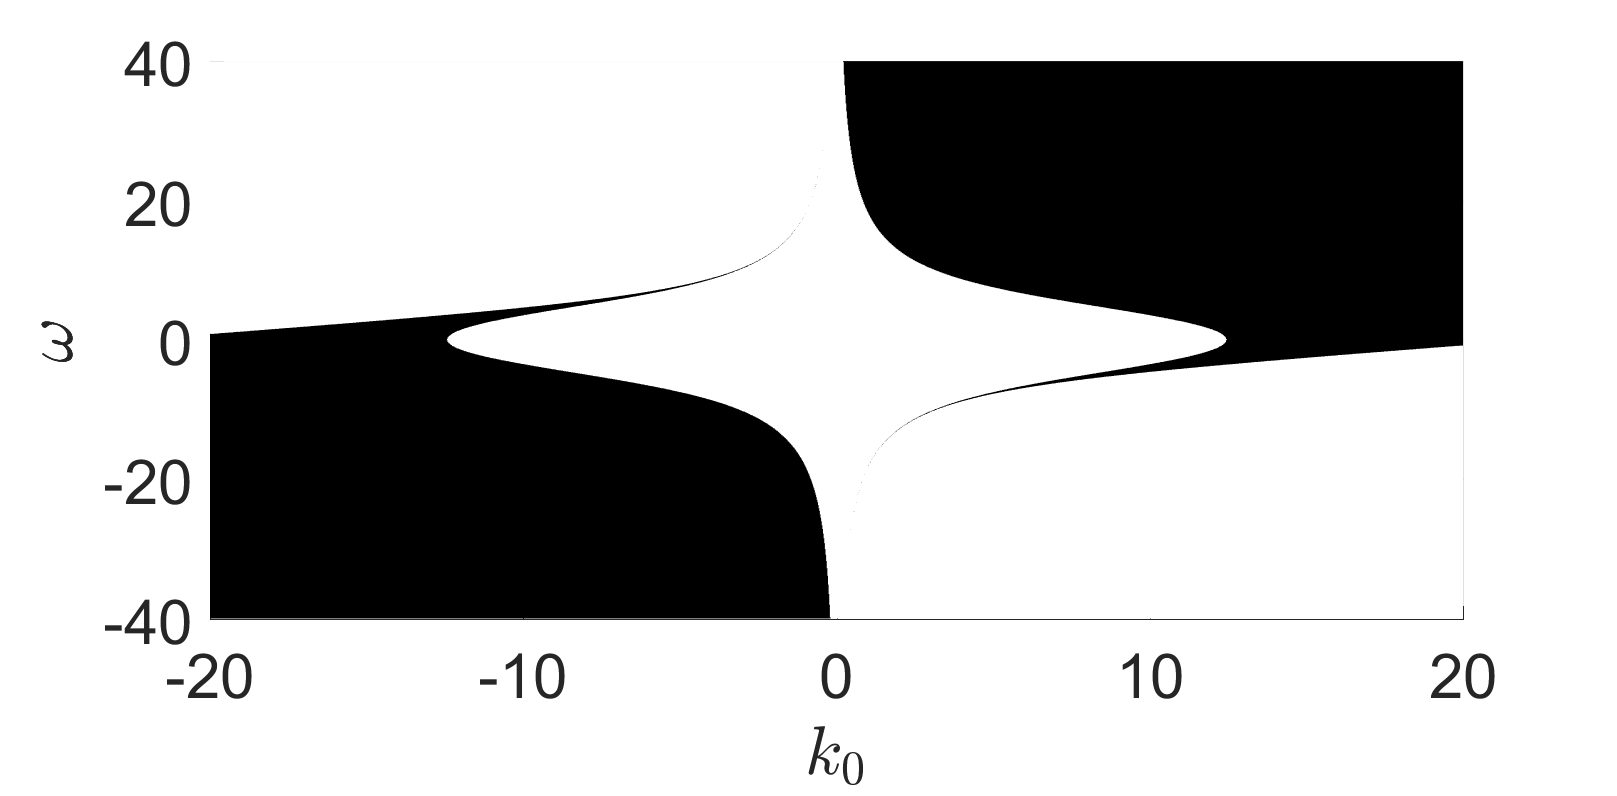
\includegraphics[width=.5\textwidth]{foc_defoc_pos_cut} & 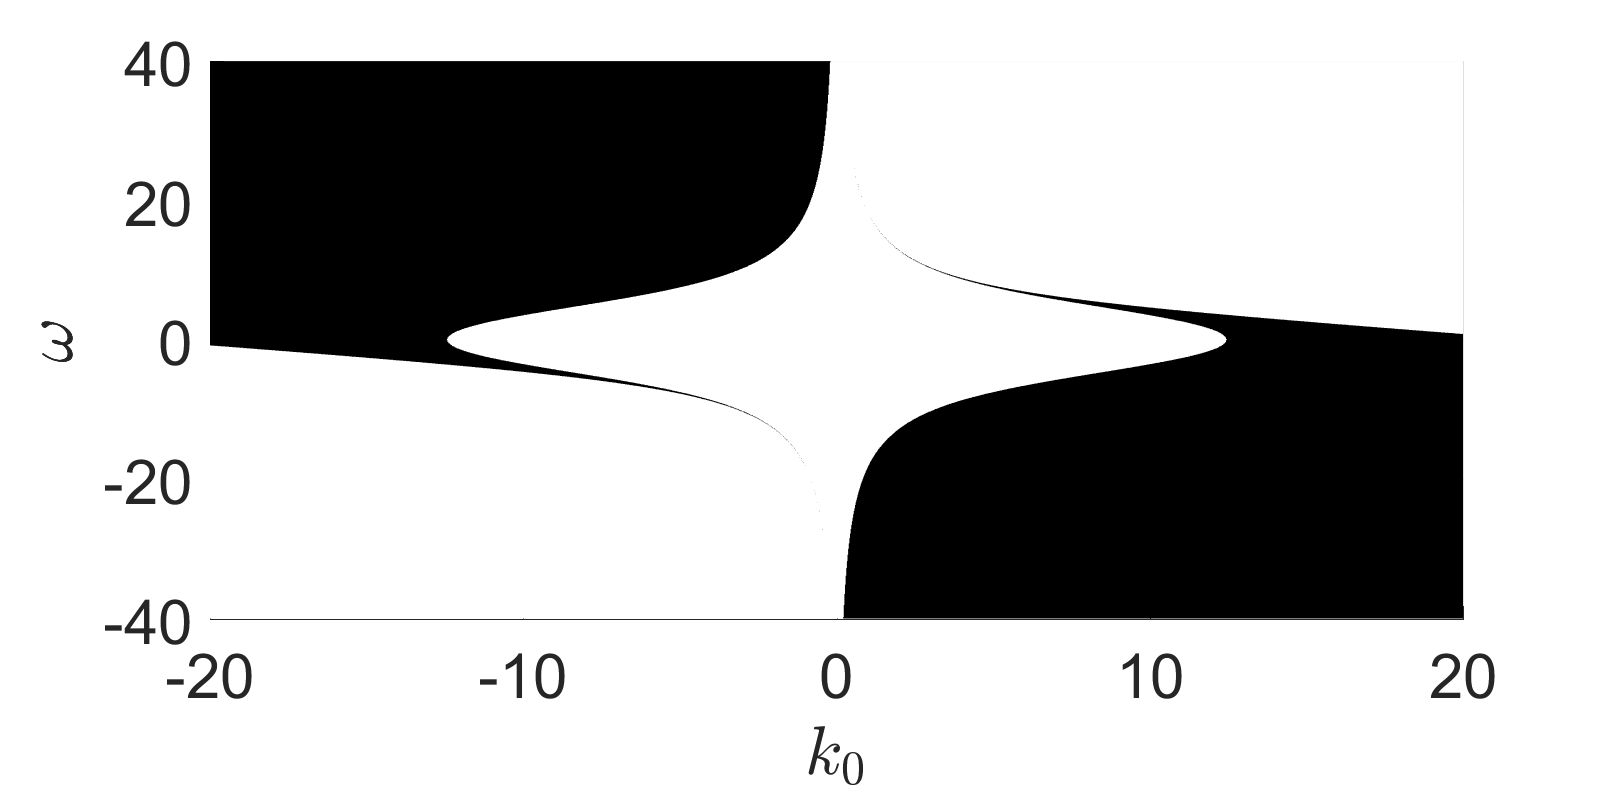
\includegraphics[width=.5\textwidth]{foc_defoc_neg_cut}\\
(a) & (b)\\
\end{tabular}
\caption{ {\it MIs exist} - white, {\it MIs suppressed} - black, for $\Omega_{+}(k_{0},\omega)$ (a) and $\Omega_{-}(k_{0},\omega)$ (b).}
\label{fig:miplot}
\end{figure}

Per our convention of taking the fast phase, $\theta(x,t)$, to be
\[
\theta(x,t) = k_{0}x + \Omega(k_{0},\omega) t,
\]
if $k_{0}>0$ and $\Omega(k_{0},\omega)>0$, then the carrier wave is propagating to the left, while if $\Omega(k_{0},\omega)<0$, it is propagating to the right.  These relationships are reversed if $k_{0}<0$.  Equation (\ref{LDR}) establishes that $\Omega_{+}(k_{0},\omega) > 0$ and $\Omega_{-}(k_{0},\omega) < 0$ for $k_{0}\neq0$.  Figures \ref{fig:miplot} (a) and (b) show that MIs are suppressed when the shear current at the surface is counter propagating to the carrier wave.  Further, these figures show that the magnitude of the shear current must increase in order for MIs to be suppressed across a wider range of carrier wave numbers $k_{0}$.  Thus, in order to suppress MIs, we need either relatively high carrier wave numbers $k_{0}$ for relatively weak shear currents, or relatively strong shear currents for relatively low carrier wave numbers. 
%%%%%%%%%%%%%%%%%%%%%%%%%%%%%%%%%%%%%%%%%%%%%%%%%%%%%%%%%%%%%%%%%%%%%%%%%%%%%%%%%%%
\subsection{Derivation of Velocity Formulas}
In non-dimensional coordinates, the position of a given fluid particle, $(x(t),z(t))$, is defined by the dynamical system 
\[
\dot{x} = \omega z + \epsilon \phi_{x}(x,z,t), ~~~~ \dot{z} = \epsilon\phi_{z}(x,z,t),
\]
\[
x(0)=x_0,~~~~ z(0)=z_0.
\]
Therefore, in order to track the motion of a fluid particle, both $\phi_x$ and $\phi_z$ must be known throughout the fluid domain.  In order to determine asymptotic formulas for these quantities, let
\begin{equation}
\phi_{x}(x,z,t) = \frac{1}{2\pi}\int_{\mathbb{R}}dk~ e^{ikx} A(k,t)e^{|k|z},
\label{phix}
\end{equation}
\begin{equation}
\phi_{z}(x,z,t) = \frac{1}{2\pi}\int_{\mathbb{R}}dk~ e^{ikx} B(k,t)e^{|k|z}.
\label{phiz}
\end{equation}
The surface boundary conditions give
\begin{align*}
\left.\phi_{x}\right|_{z=\epsilon\eta} = & \frac{Q-\epsilon\eta_{x}(\eta_{t}+\epsilon\omega\eta\eta_{x})}{1+\epsilon^{2}\eta_{x}^{2}},\\
\left.\phi_{z}\right|_{z=\epsilon\eta} = & \frac{\eta_{t}+\epsilon \left(Q+\omega\eta\right)\eta_{x}}{1+\epsilon^{2}\eta_{x}^{2}}.
\end{align*}
Therefore, with the formluas derived above, expressions for $\phi_x$ and $\phi_z$ can be found.  Assume the following asymptotic forms for the horizontal and vertical fluid velocities at the surface
\begin{align*}
\left.\phi_{x}\right|_{z=\epsilon\eta} = & \epsilon\tilde{\phi}^{(x)}_{0} + \tilde{\phi}^{(x)}_{1}e^{i\theta} +  \epsilon\tilde{\phi}^{(x)}_{2}e^{2i\theta} + \epsilon^{2}\tilde{\phi}^{(x)}_{3}e^{3i\theta} + \mbox{c.c.} + \mathcal{O}(\epsilon^{3}),\\
\left.\phi_{z}\right|_{z=\epsilon\eta} = & \epsilon\tilde{\phi}^{(z)}_{0} + \tilde{\phi}^{(z)}_{1}e^{i\theta} +  \epsilon\tilde{\phi}^{(z)}_{2}e^{2i\theta} + \epsilon^{2}\tilde{\phi}^{(z)}_{3}e^{3i\theta} + \mbox{c.c.} + \mathcal{O}(\epsilon^{3}),
\end{align*}
where
\begin{align*}
\tilde{\phi}^{(x)}_{0} = & \tilde{\phi}^{(x)}_{00} + \epsilon \tilde{\phi}^{(x)}_{01}, & ~ \tilde{\phi}^{(z)}_{0} = & \tilde{\phi}^{(z)}_{00} + \epsilon \tilde{\phi}^{(z)}_{01},\\
\tilde{\phi}^{(x)}_{1} = & \tilde{\phi}^{(x)}_{10} + \epsilon^{2} \tilde{\phi}^{(x)}_{12}, & ~ \tilde{\phi}^{(z)}_{1} = & \tilde{\phi}^{(z)}_{10} + \epsilon^{2} \tilde{\phi}^{(z)}_{12},\\
\tilde{\phi}^{(x)}_{2} = & \tilde{\phi}^{(x)}_{20} + \epsilon \tilde{\phi}^{(x)}_{21}, & ~ \tilde{\phi}^{(z)}_{2} = & \tilde{\phi}^{(z)}_{20} + \epsilon \tilde{\phi}^{(z)}_{21},
\end{align*}
and the mean terms, $\tilde{\phi}^{(x)}_{0}$ and $\tilde{\phi}^{(z)}_{0}$, are real.  The expansions are straightforward and have been done in SAGE in order to ensure accuracy.  We omit the details for the sake of brevity.

Expanding $e^{\epsilon \eta |k|}$ in equations (\ref{phix}) and (\ref{phiz}) gives
\begin{align*}
\left.\phi_{x}\right|_{z=\epsilon\eta} = & \tilde{A}(x,t) - \epsilon\eta\mathcal{H}\p_{x}\tilde{A} - \frac{\epsilon^{2}}{2}\eta^{2}\p_{x}^{2}\tilde{A} +\mathcal{O}(\epsilon^{3}),\\
\left.\phi_{z}\right|_{z=\epsilon\eta} = & \tilde{B}(x,t) - \epsilon\eta\mathcal{H}\p_{x}\tilde{B} - \frac{\epsilon^{2}}{2}\eta^{2}\p_{x}^{2}\tilde{B} +\mathcal{O}(\epsilon^{3}),
\end{align*}
where
\[
\tilde{A}(x,t) = \frac{1}{2\pi}\int_{\mathbb{R}}dk~ e^{ikx} A(k,t), ~~~~ \tilde{B}(x,t) = \frac{1}{2\pi}\int_{\mathbb{R}}dk~ e^{ikx} B(k,t).
\]
Upon inverting,
\begin{equation*}
\tilde{A}(x,t) = \epsilon\tilde{A}_{0}(\xi,\tau) + \tilde{A}_{1}(\xi,\tau) e^{i\theta} + \epsilon\tilde{A}_{2}(\xi,\tau) e^{2i\theta} + \epsilon^{2}\tilde{A}_{3}(\xi,\tau) e^{3i\theta} +\mbox{c.c}
\end{equation*}
\begin{equation*}
\tilde{B}(x,t) = \epsilon\tilde{B}_{0}(\xi,\tau) + \tilde{B}_{1}(\xi,\tau) e^{i\theta} + \epsilon\tilde{B}_{2}(\xi,\tau) e^{2i\theta} + \epsilon^{2}\tilde{B}_{3}(\xi,\tau) e^{3i\theta} + \mbox{c.c},
\end{equation*}
where the mean terms, $\tilde{A}_{0}$ and $\tilde{B}_{0}$, are real.
Then, using the facts that
\[
A(k,t) = \int_{\mathbb{R}}dx~ e^{-ikx} \tilde{A}(x,t), ~~~~ B(k,t) =
\int_{\mathbb{R}}dx~ e^{-ikx} \tilde{B}(x,t),
\]
$\phi_{x}(x,z,t)$ and $\phi_{z}(x,z,t)$ can be approximated via the expansions
\[
\phi_{x}(x,z,t) = \tilde{\phi}_{x}(x,z,t) + \mathcal{O}(\epsilon^{3}), ~ \phi_{z}(x,z,t) = \tilde{\phi}_{z}(x,z,t) + \mathcal{O}(\epsilon^{3}),
\]
where 
\begin{equation}
\tilde{\phi}_{x}(x,z,t) = \epsilon R_{0}(\xi,Z,\tau) + R_{1}(\xi,z,\tau)e^{i\theta} \\+ \epsilon R_{2}(\xi,z,\tau)e^{2i\theta} + \epsilon^{2}R_{3}(\xi,z,\tau)e^{3i\theta} + \mbox{c.c.},
\label{phixexp}
\end{equation}
\begin{equation}
\tilde{\phi}_{z}(x,z,t) = \epsilon \tilde{R}_{0}(\xi,Z,\tau) + \tilde{R}_{1}(\xi,z,\tau)e^{i\theta} \\+ \epsilon \tilde{R}_{2}(\xi,z,\tau)e^{2i\theta} 
+ \epsilon^{2}\tilde{R}_{3}(\xi,z,\tau)e^{3i\theta} + \mbox{c.c.}.
\label{phizexp}
\end{equation}
Again, while the expansion procedure is straightforward, due to the length of the expressions involved, the details have been ommitted.



%%%%%%%%%%%%%%%%%%%%%%%%%%%%%%%%%%%%%%%%%%%%%%%%%%%%%%%%%%%%%%%%%%%%%%%%%%%%%%%%%%%
\section{Stokes Drift}
Following the Generalized Lagrangian Mean (GLM) formalism presented in
\cite{andrews}, for some quantity $\varphi({\bf x},t)$, given an
Eularian mean operator $\bar{()}$, we define the Lagrangian mean
$\bar{()}^{L}$ at a point ${\bf x}$ relative to the disturbance ${\bf
  y}({\bf x},t)$ to be  
\[
\bar{\varphi}^{L}({\bf x},t) = \overline{\varphi({\bf x}+{\bf y}({\bf x},t),t)}.
\]
Assuming the mapping ${\bf x} + {\bf y}$ where
\[
{\bf x} + {\bf y}({\bf x},t) = \left(x+y_{1}(x,z,t),z+y_{2}(x,z,t)\right),
\]
is a diffeomorphism, then a corresponding Lagrangian averaged speed, say $\overline{{\bf u}}^{L}({\bf x},t)$, is defined by the equation
\begin{equation}
\left(\p_{t} + \overline{{\bf u}}^{L}({\bf x},t)\cdot \nabla_{{\bf x}} \right) \left({\bf x} + {\bf y}({\bf x},t)\right) = {\bf u}\left({\bf x} + {\bf y}({\bf x},t),t\right).
\label{speeddef}
\end{equation}
The other requirements in the GLM formalism are that 
\begin{align*}
\overline{{\bf y}({\bf x},t)} = & \bf{0}, \\
\overline{\overline{{\bf u}}^{L}({\bf x},t)} = & \overline{{\bf u}}^{L}({\bf x},t).
\end{align*}
Throughout the remainder of this paper, the Eularian average will be
given by integration with respect to the fast phase variable $\theta$,
i.e.  
\[
\bar{f}(\xi,z,\tau) = \frac{1}{2\pi}\int_{0}^{2\pi} d\theta~ f(\xi,z,\tau,\theta).
\]
Having chosen the averaging operator, one should read the requirement $\overline{{\bf y}}=0$ as in effect a definition of the disturbance.  But it should be emphasized that the GLM formalism is powerful specifically because of the degree of flexibility it provides in defining what the mean and fluctuation components of a flow are.   Using the above definitions, the Stokes drift, $\varphi^{S}({\bf x},t)$, of a quantity $\varphi$ can be unambiguously defined to be 
\[
\varphi^{S}({\bf x},t) = \overline{\varphi}^{L}({\bf x},t) - \overline{\varphi({\bf x},t)}. 
\]
%Throughout GLM, in order to get explicitly computable quantities, some approximation must be made.  

Since we defined the averaging operator to be integration with respect to the fast phase $\theta$, the Eularian mean of the horizontal velocity $u({\bf x},t)$ is  
\[
\overline{u}({\bf x},t) = \omega z + \overline{u}_{i}(\xi,Z,\tau), 
\]
where the irrotational average velocity $\overline{u}_{i}$ is given by 
\[
\overline{u}_{i}(\xi,Z,\tau) = \epsilon^{2}R_{0}(\xi,Z,\tau) + \mathcal{O}(\epsilon^{3}).
\]
Define the Eularian horizontal fluctuation speed $u'({\bf x},t)$ to be
\[
u'({\bf x},t) = \epsilon\left(e^{i\theta}R_{1} + e^{-i\theta}R_{1}^{\ast} \right)
+  \epsilon^{2}\left( e^{2i\theta}R_{2} + e^{-2i\theta}R_{2}^{\ast}\right)  + \mathcal{O}(\epsilon^{3}).
\]
This implies that the horizontal fluid velocity $u$ can be written in the form 
\[
u({\bf x},t) = \omega z +  u'({\bf x},t) + \bar{u}_{i}(\xi,Z,\tau).
\]
It is then consistent to suppose that the disturbance ${\bf y}=\mathcal{O}(\epsilon)$, so that
\begin{align*}
\overline{u}^{L}({\bf x},t) = & \overline{u({\bf x} + \epsilon {\bf y},t)} \\
= & \overline{\omega (z + \epsilon y_{2}) +  u'({\bf x},t) + \bar{u}_{i}(\xi,Z,\tau) + \epsilon (y_{1}\p_{x}u' + y_{2}\p_{z}u') + \mathcal{O}(\epsilon^{3})} \\
= & \omega z + \bar{u}_{i}(\xi,Z,\tau) + \epsilon \overline{(y_{1}\p_{x}u' + y_{2}\p_{z}u')} + \mathcal{O}(\epsilon^{3}).
\end{align*}
Note that since the disturbance must have zero Eularian average, the
shear current $\omega z$ cannot directly contribute to Stokes drift
since
\[
\overline{\omega\left(z + \epsilon y_{2}({\bf x},t)\right)} = \omega z,
\]
and thus $\omega z$ must be a common term to both $\overline{u}^{L}$ and $\overline{u}$.  Likewise,
\[
\overline{u}^{L}({\bf x},t) = \omega z + \mathcal{O}(\epsilon^{2}).
\]
Using identical arguments for the vertical velocity, $w({\bf x},t)$ gives 
\[
w({\bf x},t) = w'({\bf x},t) + \bar{w}_{i}(\xi,Z,\tau),
\]
where $w'=\mathcal{O}(\epsilon)$ and $\bar{w}_{i}=\mathcal{O}(\epsilon^{2})$.  This implies that the Lagrangian mean of the vertical velocity $\overline{w}^{L}({\bf x},t) = \mathcal{O}(\epsilon^{2})$.

Equation \eqref{speeddef} establishes that
\[
\p_{t}{\bf y} + \omega z \p_{x}{\bf y} - \omega \bp y_{2}\\ 0 \ep = \bp R_{1}e^{i\theta}+R^{\ast}_{1}e^{-i\theta}\\ \tilde{R}_{1}e^{i\theta}+\tilde{R}^{\ast}_{1}e^{-i\theta} \ep + \mathcal{O}(\epsilon).
\]
Treating the value $z$ as an Eularian parameter, the method of characteristics gives 
\begin{align*}
y_{1} = & - \frac{i}{k_{0}\omega z + \Omega}\left(R_{1}e^{i\theta} -R^{\ast}_{1}e^{-i\theta} \right) - \frac{\omega}{(k_{0}\omega z + \Omega)^{2}}\left(\tilde{R}_{1}e^{i\theta} + \tilde{R}^{\ast}_{1}e^{-i\theta} \right)\\
y_{2} = & - \frac{i}{k_{0}\omega z + \Omega}\left(\tilde{R}_{1}e^{i\theta} -\tilde{R}^{\ast}_{1}e^{-i\theta} \right)
\end{align*}
Following the GLM formalism, the horizontal Stokes drift velocity $u^{S}(x,z,t)$ is given by 
\begin{align*}
u^{S}(x,z,t) = & \epsilon \left(\overline{y_{1}u'_{x}} + \overline{y_{2}u'_{z}}\right)  + \mathcal{O}(\epsilon^{3})\\
= & \epsilon \left(\overline{y_{1}u'_{x}} + \overline{y_{2}w'_{x}}\right)  + \mathcal{O}(\epsilon^{3})\\
= & \frac{2\epsilon^{2}}{c_{p}-\omega z}\left(\left|R_{1}\right|^{2} + \left|\tilde{R}_{1}\right|^{2} + \frac{\omega}{k_{0}(c_{p}-\omega z)}\mbox{Im}\left\{R_{1}\tilde{R}_{1}^{\ast}\right\} \right) + \mathcal{O}(\epsilon^{3}),
\end{align*}
where the phase speed $c_{p}$ is given by 
\[
c_{p}(k_{0},\omega) = -\frac{\Omega_{\pm}(k_{0},\omega)}{k_{0}},
\]
and where we have used the irrotationality of the velocity fluctuations $(u',w')$ to derive the second line.  Due to our choice of signs in $\theta(x,t)$, we use the opposite sign on the phase speed so that a positive phase speed $c_{p}$ corresponds to a rightward propagating phase.  

In the case of a plane-wave solution, the Stokes drift velocity at the surface can be evaluated in closed form giving  
\begin{equation}
u^{S}(x,z,t) = \frac{2\epsilon^{2}A^{2}\Omega^{2}}{c_{p}-\omega z} \left(2  + \frac{\omega}{|k_{0}|(c_{p}-\omega z)} \right) e^{2|k_{0}|z} + \mathcal{O}(\epsilon^{3}).
\label{pwavesdrift}
\end{equation}
This expands on the classic result for the Stokes drift over infinitely deep water, and shows how constant shear currents modify the drift speed.

%%%%%%%%%%%%%%%%%%%%%%%%%%%%%%%%%%%%%%%%%%%%%%%%%%%%%%%%%%%%%%%%%%%%%%%%%%%%%%%%%%%
%%%%%%%%%%%%%%%%%%%%%%%%%%%%%%%%%%%%%%%%%%%%%%%%%%%%%%%%%%%%%%%%%%%%%%%%%%%%%%%%%%%
\section{Numerical Results}
Given that the solutions to the NLS equation are in terms of the coordinates $\xi$ and $\tau$, we use a fourth-order Runge-Kutta scheme with a time step of $\delta \tau = 10^{-3}$ to solve the dynamical system
\[
\frac{d \xi_{s}}{d\tau} =  \frac{c_{g}}{\epsilon} + \frac{\omega}{\epsilon}z_{s} + \tilde{\phi}_{x}(\xi_{s},z_{s}), ~ \frac{dz_{s}}{d\tau} = \frac{1}{\epsilon} \tilde{\phi}_{z}(\xi_{s},z_{s}),
\]
where $\tilde{\phi}_{x}$ and $\tilde{\phi}_{z}$ are the truncated potentials in equations \eqref{phixexp} and \eqref{phizexp} respectively.  We choose the initial tracer position to be 
\[
\xi_{s}(0) = \frac{K(\kappa)}{128}, ~ z_{s}(0) = \epsilon \tilde{\eta}(\xi_{s}(0),0),
\]
where $K(\kappa)$ is the complete elliptic integral of the first kind, and $\tilde{\eta}$ is found via the expansion in Equation \eqref{nlssurfexpan}.  We take the positive branch, $\Omega_{+}$, of the dispersion relationship.  The results for the tracer position, $(x_{s}(t),z_{s}(t))$, are found using the transformations 
\[
x_{s}(t) = \frac{\xi_{s}(\tau)}{\epsilon}-\frac{c_{g}\tau}{\epsilon^{2}}, ~ t = \frac{\tau}{\epsilon^{2}}.
\]
Fourier transforms are done numerically using the fast Fourier transform.  Similarly, inverse transforms used to compute $R_{j}$ and $\tilde{R}_{j}$ in equations \eqref{phixexp} and \eqref{phizexp} are also computed using the fast Fourier transform.  Throughout this section, we choose $\tilde{\sigma} = 10^{-3}$, which is a physically reasonable value.  Throughout the remainder of the text, we report results on the Stokes velocity in terms of the rescaled velocity $\tilde{u}^{S}$ where 
\[
\tilde{u}^{S} = \frac{u^{S}}{\epsilon^{2}}.
\]
We ignore the $\epsilon^{2}$ scaling term since this parameter does not play any role in the effect that different shear currents have on the transport properties of surface waves. 

Before presenting results, we address the accuracy of our approach.  The original fluid model requires that particles which start on the fluid surface remain there, while the NLS equation only approximately satisfies this constraint.  In order to examine this relationship, consider
\[
\mathcal{E}(\epsilon,\omega) = \epsilon^{2}\int_{0}^{1/\epsilon^{2}}\big{|}z_{s}(t) - \epsilon\eta(x_{s}(t),t) \big{|}dt, 
\]    
where the asymptotic expansion for $\eta$ in equation \eqref{nlssurfexpan} is used.  This is an average of the difference between the surface location and the particple location.  (If $\mathcal{E}\epsilon,\omega)=0$, then the particle started on the surface and remained there over the interval $t\in[0,1/\epsilon^2$.  Table \ref{errtab} where where $\mathcal{E}_{j}(0) = \mathcal{E}(\epsilon_{j},0)$ was created using the focusing NLS solution with elliptic modulus $\kappa = 0.5$.
\begin{table}[!h]
\centering
\begin{tabular}{c|cccccc}
$\epsilon_{j}=2^{-j}$ & $\mathcal{E}_{j}(0)$ & $\mathcal{E}_{j}(1)$ & $\mathcal{E}_{j}(-1)$ & $\frac{\mathcal{E}_{j-1}(0)}{\mathcal{E}_{j}(0)}$ & $\frac{\mathcal{E}_{j-1}(1)}{\mathcal{E}_{j}(1)}$ & $\frac{\mathcal{E}_{j-1}(-1)}{\mathcal{E}_{j}(-1)}$\\ 
\hline
1/4 & 0.0012 & 8.3502e-04 & 7.0686e-04 & & & \\
1/8 & 2.6800e-04 & 1.9854e-04 & 9.9677e-05 & 4.4776 & 4.207 & 7.092\\
1/16 & 7.2528e-05  & 5.3587e-05 & 1.7080e-05 & 3.695 & 3.705 & 5.836 \\
1/32 & 1.6383e-05 & 1.0200e-05 & 3.5684e-06 & 4.4270 & 5.254 & 4.787
\end{tabular}
\caption{Error results for several values of $\epsilon$ in the focusing NLS case with elliptic modulus $\kappa=0.5$.}
\label{errtab}
\end{table}
To interpret these results, using the exact equation $\dot{z}=\epsilon\phi_{z}$ along with the approximation to $\phi_{z}$ in equation \eqref{phizexp}, gives
\[
 \dot{z} = \epsilon\tilde{\phi}_{z} + \epsilon^{4}\tilde{R}_{4}(t),
\] 
where the remainder of the expansion as $\tilde{R}_{4}(t)$ has been explicitly included.  Per the assumptions that are used in deriving NLS, suppose that there exists some positive constant $M_{\epsilon}$ such that 
\[
\left|\tilde{R}_{4}(t) \right|\leq M_{\epsilon}, ~ t \lesssim \mathcal{O}(1/\epsilon^{2}). 
\]
If the real fluid surface at $x_{s}(t)$ is given by $z(t) = \epsilon \eta(x_{s}(t),t)$, using Equation \eqref{nlssurfexpan} gives
\[
z(t) = \epsilon\tilde{\eta}(x_{s}(t),t) + \mathcal{O}(\epsilon^{4}).
\]
After integrating over $t\in[0,1/\epsilon^{2}]$, the time scale over which NLS is valid, the error in the vertical position due to the remainder is given by
\begin{align*}
\left|z_{s}(1/\epsilon^{2})-\epsilon\tilde{\eta}(x_{s}(1/\epsilon^{2}),1/\epsilon^{2})\right| \leq & \epsilon^{4}\int_{0}^{1/\epsilon^{2}}\left|\tilde{R}_{4}(t)\right| dt + \mathcal{O}(\epsilon^{4}),\\
\leq & \epsilon^{2}M_{\epsilon} + \mathcal{O}(\epsilon^{4}) = \mathcal{O}(\epsilon^{2}).
\end{align*}
The error results in Table \ref{errtab} are consistent with this bound.   As seen, this holds over different values of the vorticity as well, and thus we have confidence that our numerics are correct.  Similar results were obtained for the case $\kappa=.99$ across the same range of vorticity values, thus adding even further confirmation that our expansions and numerics are accurate.
%%%%%%%%%%%%%%%%%%%%%%%%%%%%%%%%%%%%%%%%%%%%%%%%%%%%%%%%%%%%%%%%%%%%%%%%%%%%%%%%%%% 
\subsection{Focusing Case}
Using the solution given in equation \eqref{cnsolns} with $k_0=1$ ensures that $\omega = 0$ and $\omega=\pm 1$ are in the focusing case.   Figure \ref{fig:foc_kap_pt5} was generated by setting $\epsilon=0.1$, $\kappa=0.5$, and solving the dynamical system for the particle paths up to time $t=1/\epsilon^{2}$.  The leading-order carrier profile is propagating to the left.  Therefore, if $\omega=1$, then the shear current is counter-propagating with respect to the carrier wave while for $\omega=-1$, the current is co-propagating.  The counter-propagating current severly restricts the horizontal motion of a tracer along the surface as seen by comparing Figures \ref{fig:foc_kap_pt5} (b) and (c) with (a).  The co-propagating current, i.e. $\omega=-1$, reduces the vertical displacement of the surface particle while slightly reducing the net horizontal drift of the tracer, which we expect since $\dot{x}\sim \omega z$.    

\begin{figure}
\centering
\begin{tabular}{cc}
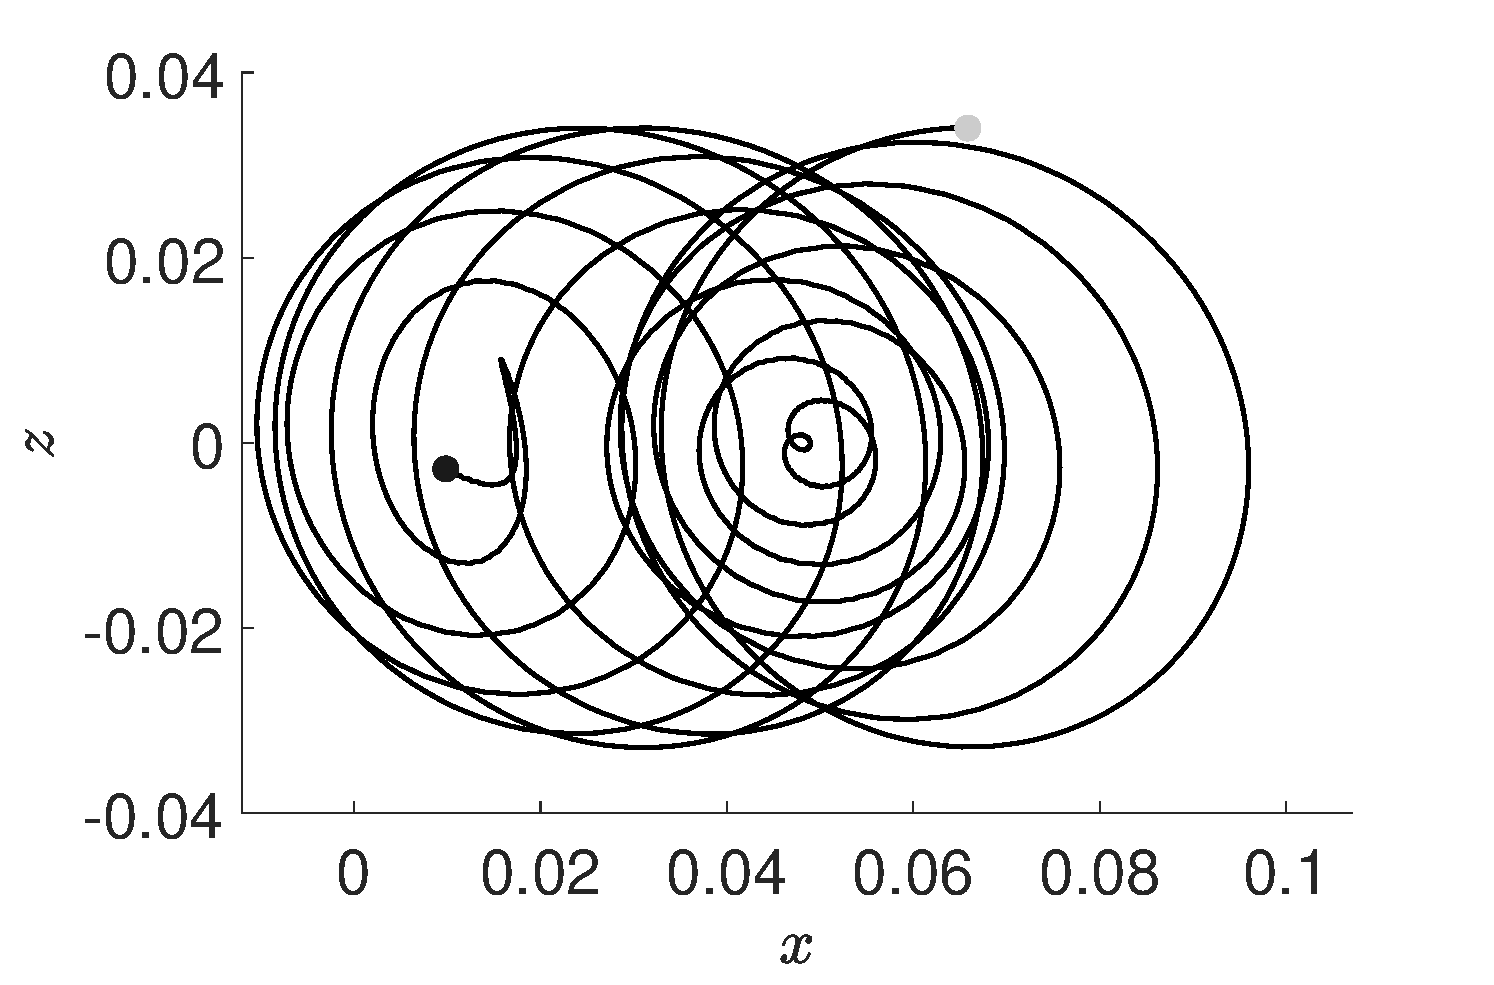
\includegraphics[width=.48\textwidth]{track_ep_pt1_tf_1_w_0_kap_pt5_foc} & 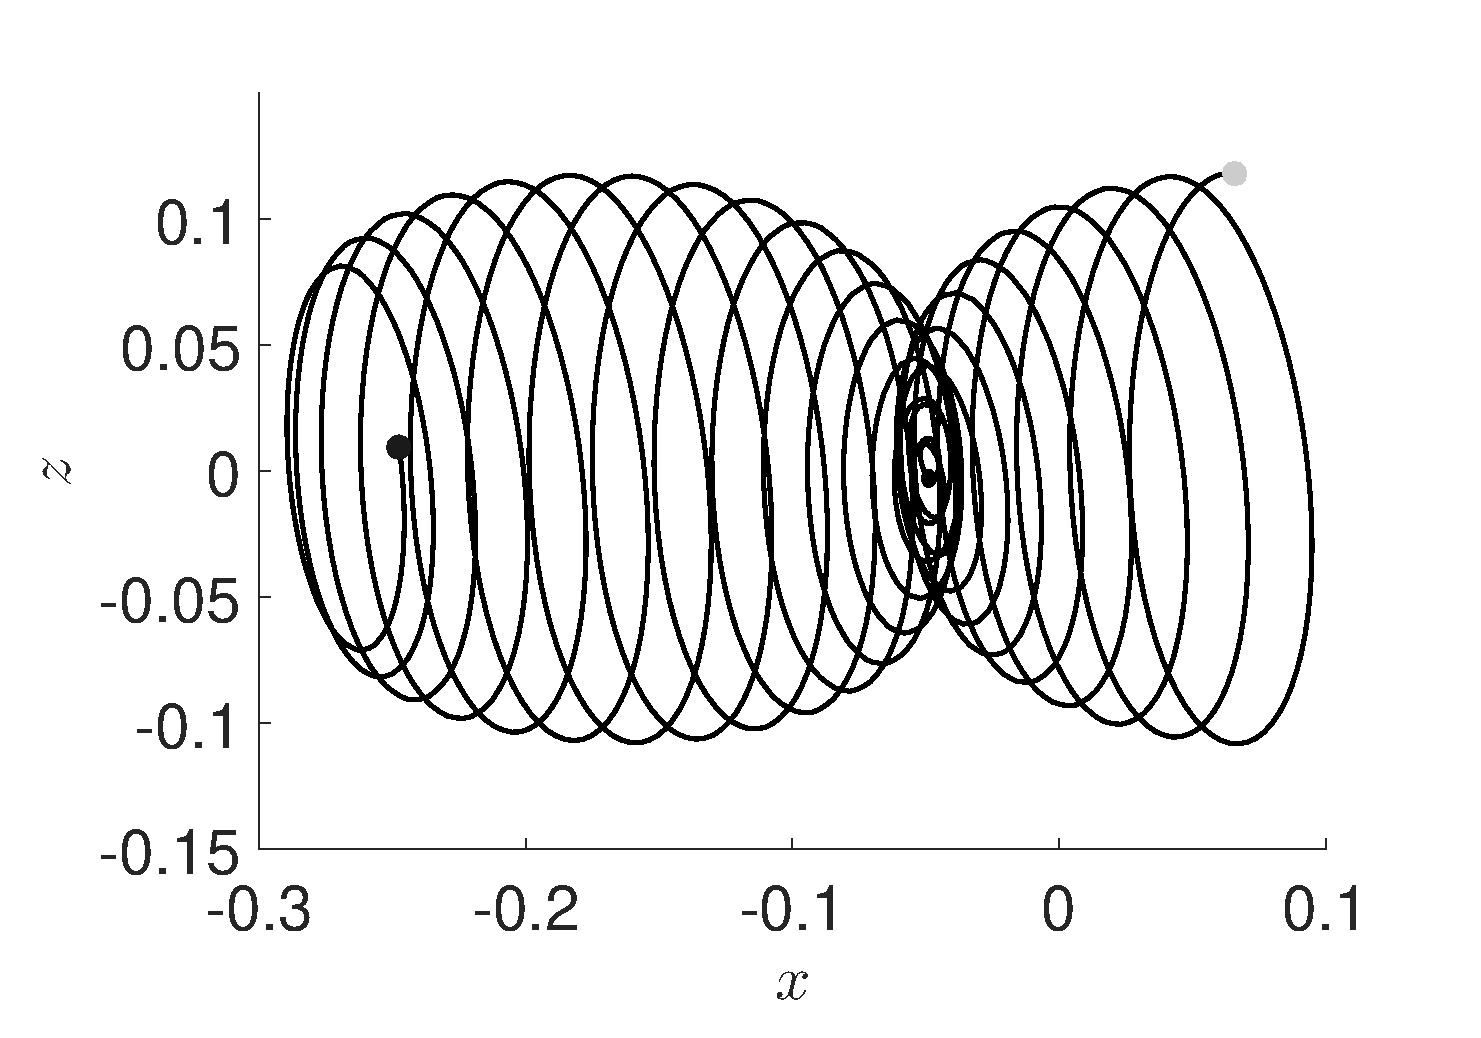
\includegraphics[width=.48\textwidth]{track_ep_pt1_tf_1_w_1_kap_pt5_foc} \\
(a) $\omega=0$ & (b) $\omega=1$\\ 
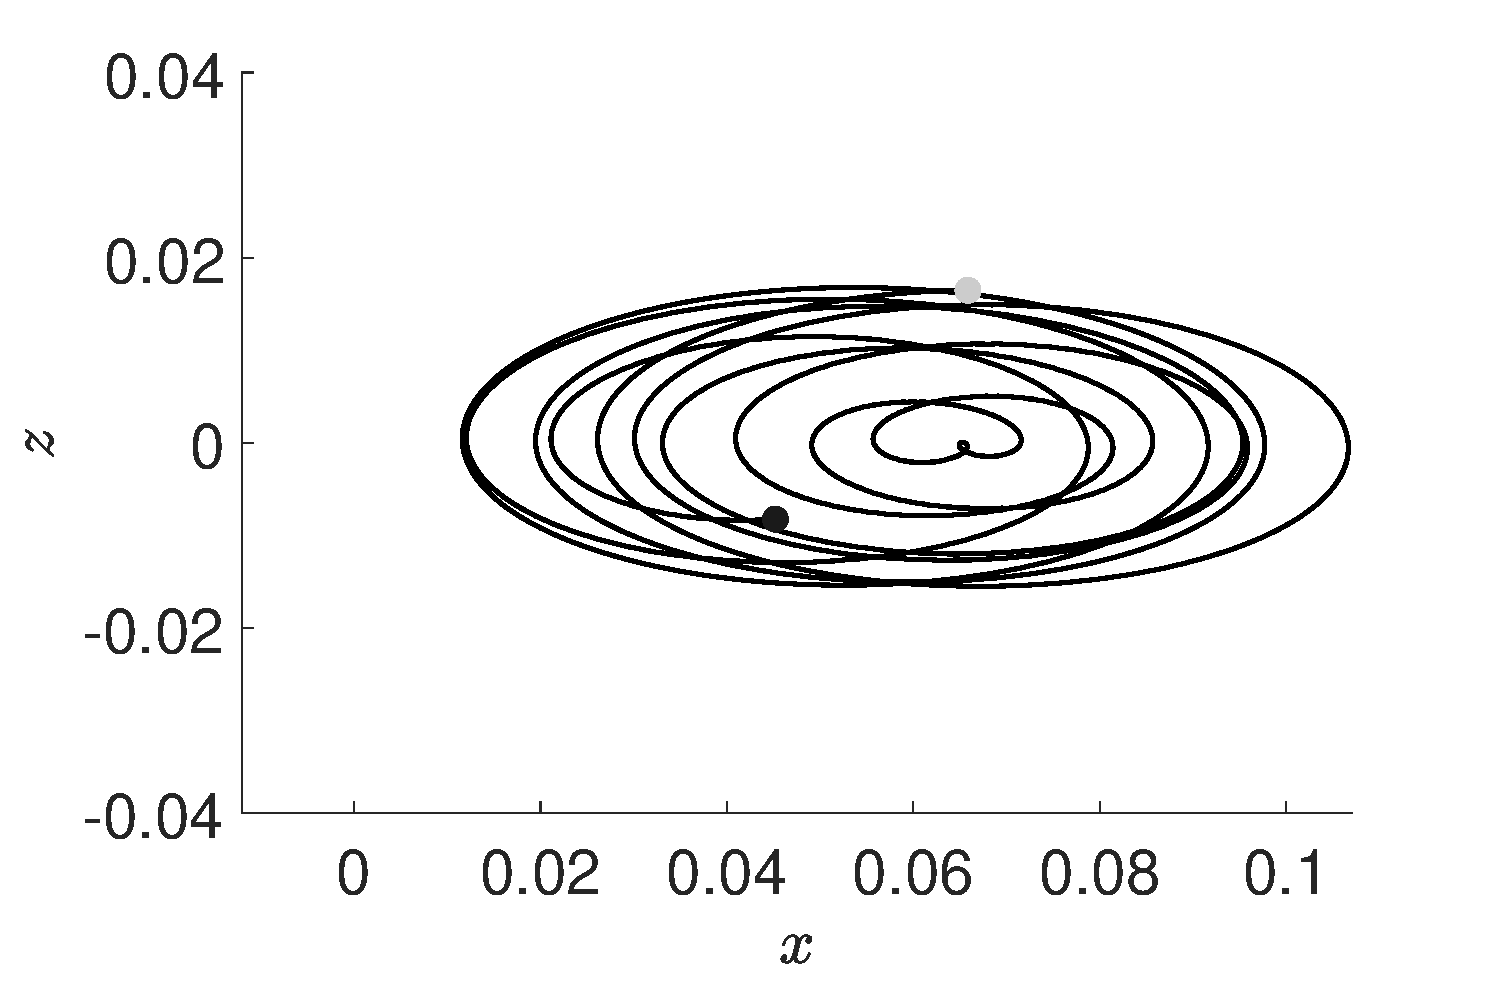
\includegraphics[width=.48\textwidth]{track_ep_pt1_tf_1_w_n1_kap_pt5_foc} & 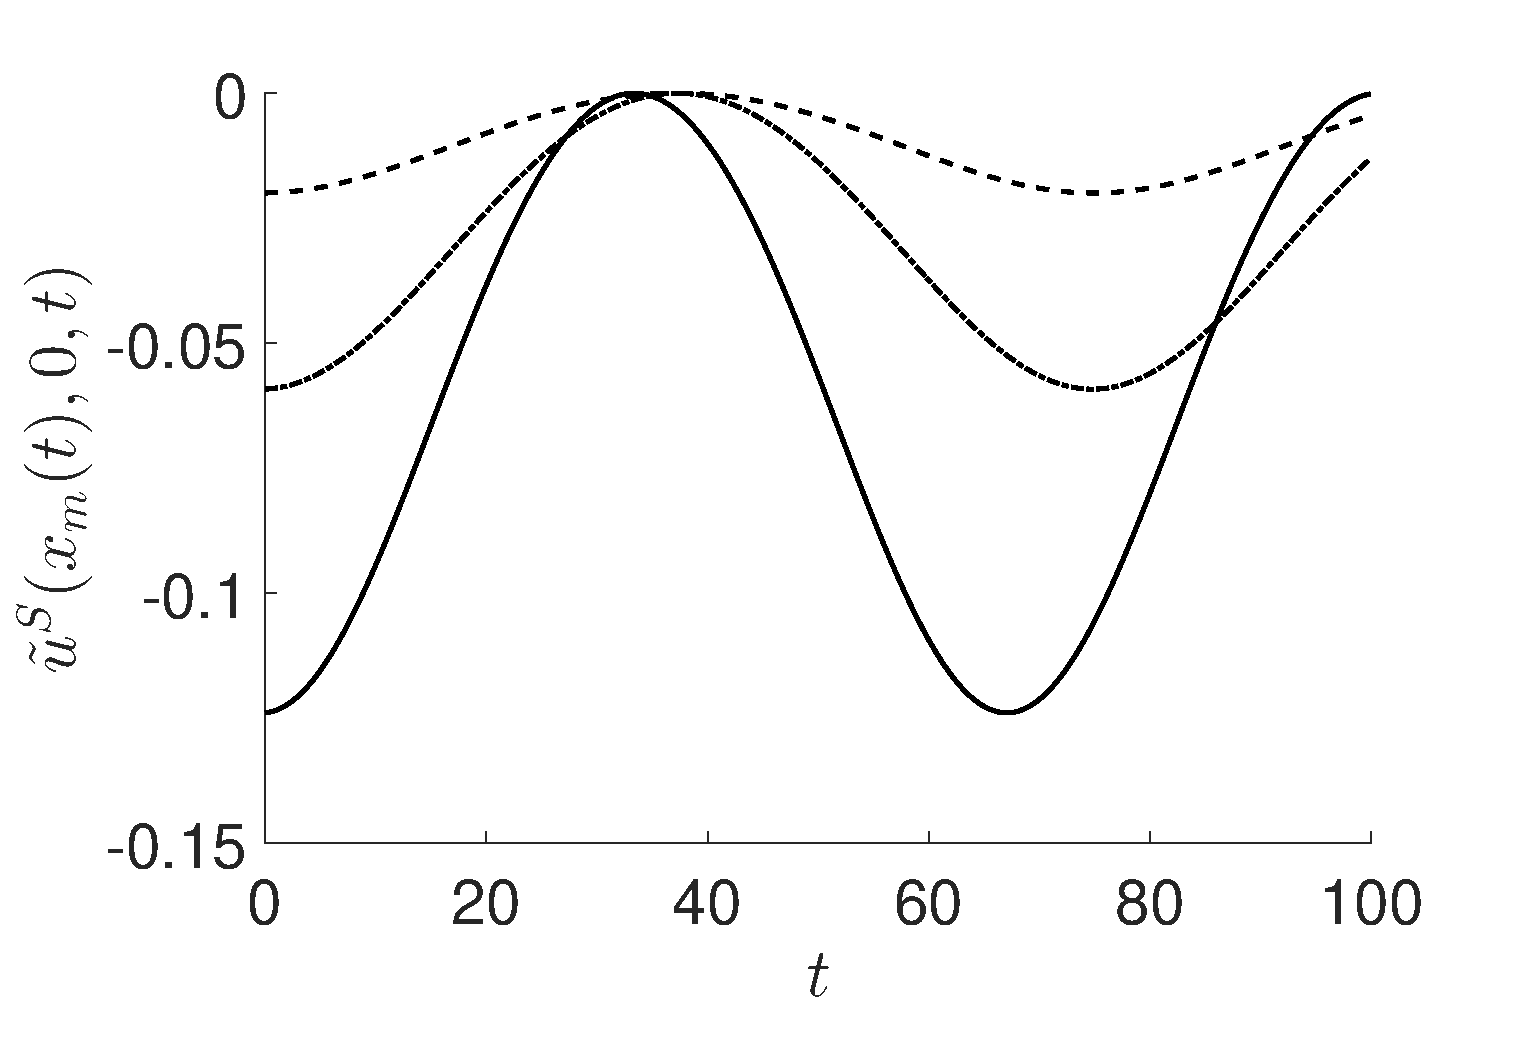
\includegraphics[width=.48\textwidth]{sdrift_comp_ep_pt1_tf_1_kap_pt5_foc}\\
(c) $\omega=-1$ & (d) Stokes Velocity\\
\end{tabular}
\caption{{\bf Focusing} - $k_{0}=1$, $\kappa=0.5$, $\omega=0$ (a), $\omega=1$ (b), and $\omega=-1$ (c), Stokes velocity $\tilde{u}^{S}$ (d), where $\omega=0$ (--), $\omega=1$ (-.), and $\omega=-1$ (- -). The grey dots indicate the starting positions of the tracers while the black dots indicate their final positions.}
\label{fig:foc_kap_pt5}
\end{figure}

Figure \ref{fig:foc_kap_pt5} (d) shows that the Stokes velocity is negative for all three choices of the constant vorticity.  This reflects the overall tendency of the waves to travel to the left.  Further, the Stokes velocity is significantly reduced in the presence of the counter-propagating shear current.  The greatest reduction in the Stokes velocity comes from the co-propagating shear current when $\omega=-1$.  This is explained in Figure \ref{fig:amfoc}, which includes a plot of $\sqrt{2\alpha_{d}/\alpha_{nl}}$ as a function of $\omega$.  Equation \eqref{cnsolns} shows that this term is the key factor in determining the amplitude of the surface profile for a fixed value of the elliptic modulus.  As seen, all of the choices of vorticity lessen the amplitude of the function, but the counterpropagating case causes the greatest attenuation.  
\begin{figure}
\centering
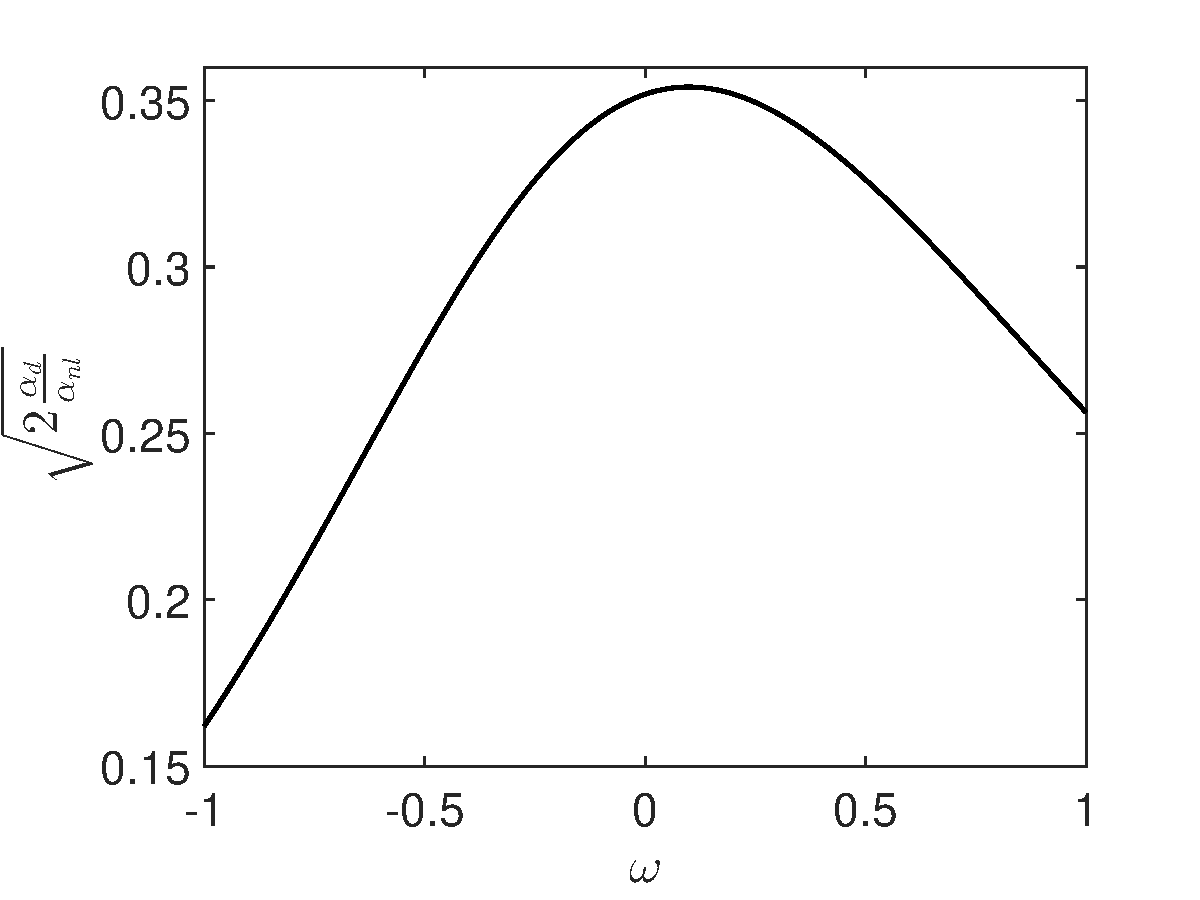
\includegraphics[width=.48\textwidth]{amp_factor_k0_1_foc}
\caption{{\bf Focusing} - The term $\sqrt{2\alpha_{d}/\alpha_{nl}}$ as a function of $\omega$ for $k_{0}=1$.}
\label{fig:amfoc}
\end{figure}
We point out though that the leading order shear current is not accounted for in the computation of the Stokes velocity since it is a common term in both the mean Lagrangian and Eularian fluid velocity descriptions.  Thus, we see that the net leftward drift seen in Figure \ref{fig:foc_kap_pt5} (c) is due to the shear.  This shear otherwise supresses the leftward drift due to the Stokes velocity when $\omega=0$; see Figure \ref{fig:foc_kap_pt5} (a) and (d).  Thus, it appears that in some sense, either the Stokes velocity or the shear is the active means for transport, but they cannot both be active at the same time.  

\begin{figure}
\centering
\begin{tabular}{cc}
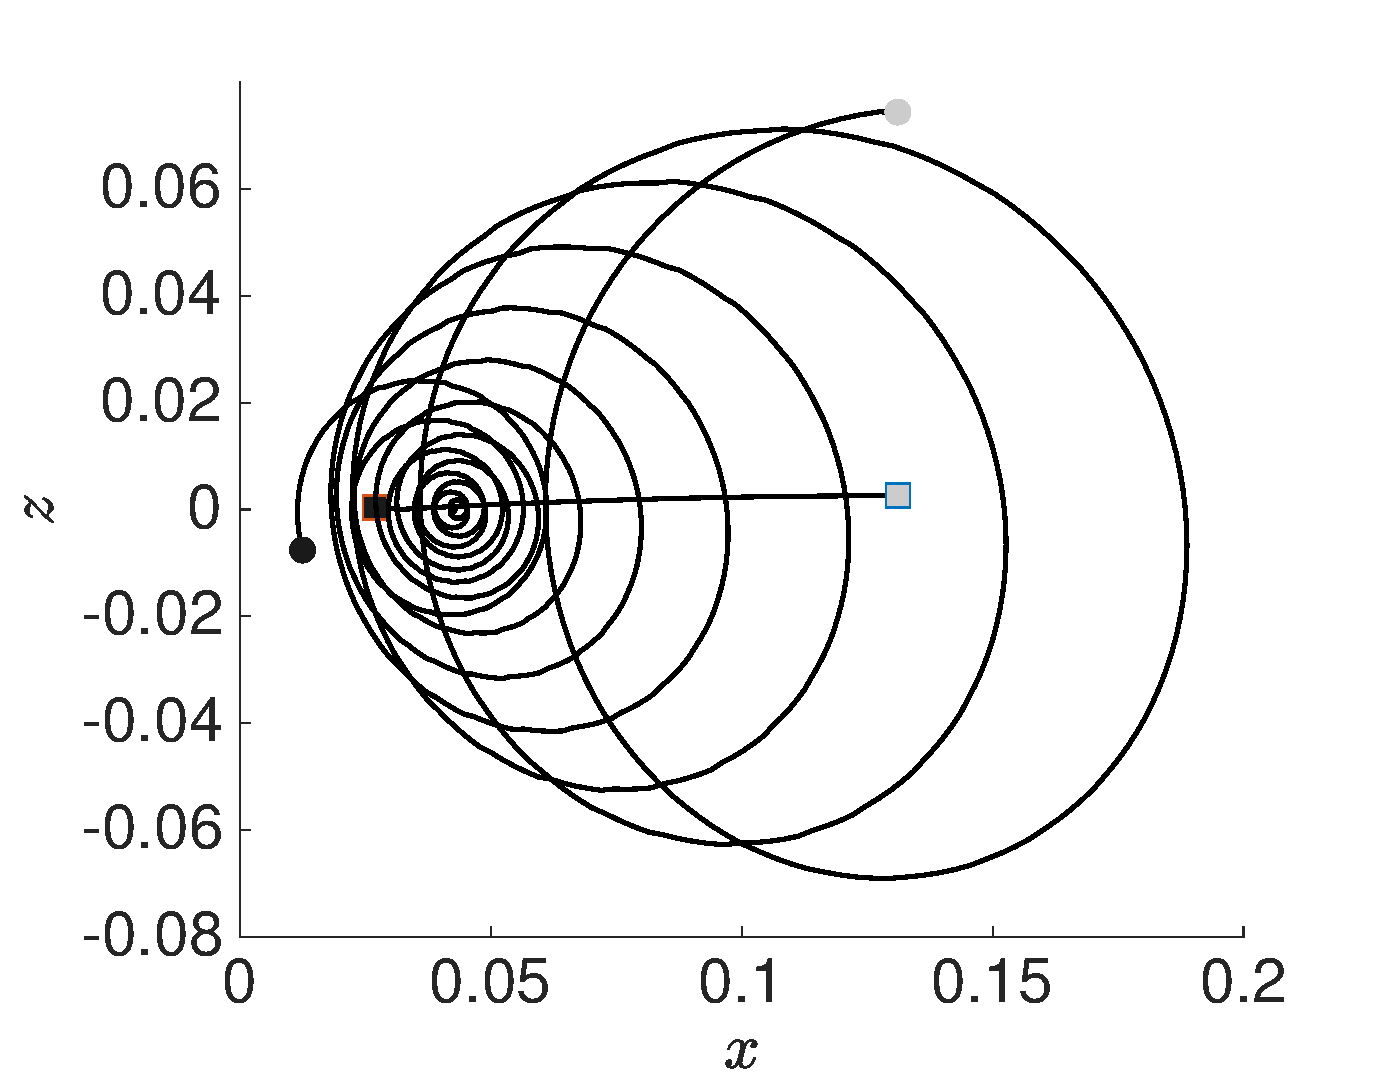
\includegraphics[width=.48\textwidth]{track_ep_pt1_tf_1_w_0_kap_pt99_foc} & 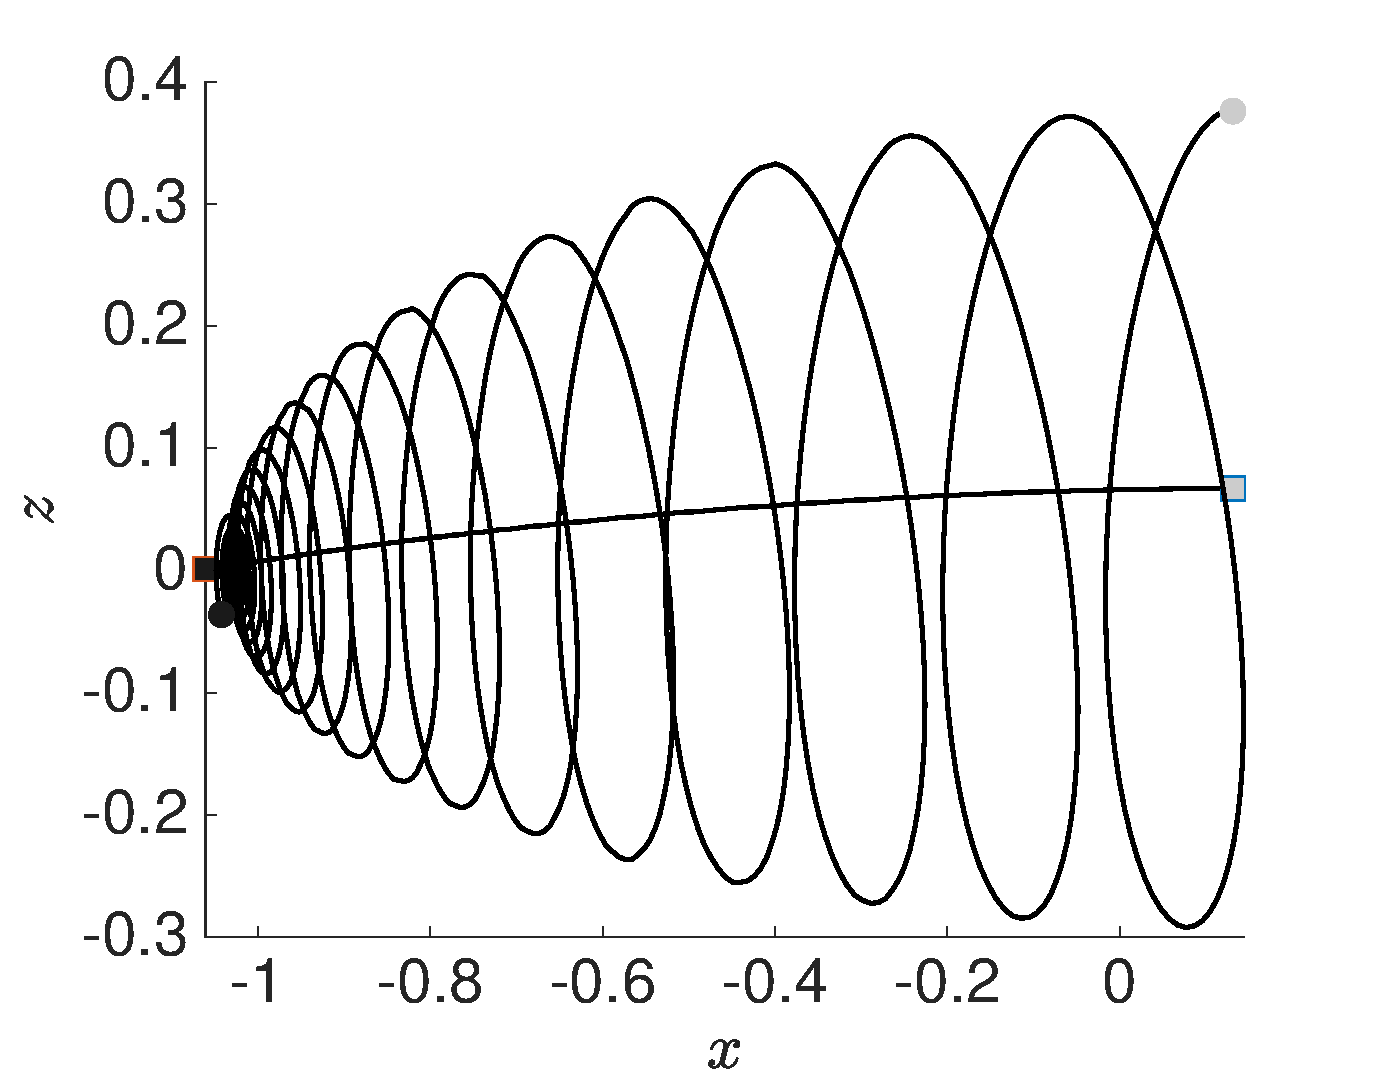
\includegraphics[width=.48\textwidth]{track_ep_pt1_tf_1_w_1_kap_pt99_foc} \\
(a) $\omega=0$ & (b) $\omega=1$\\ 
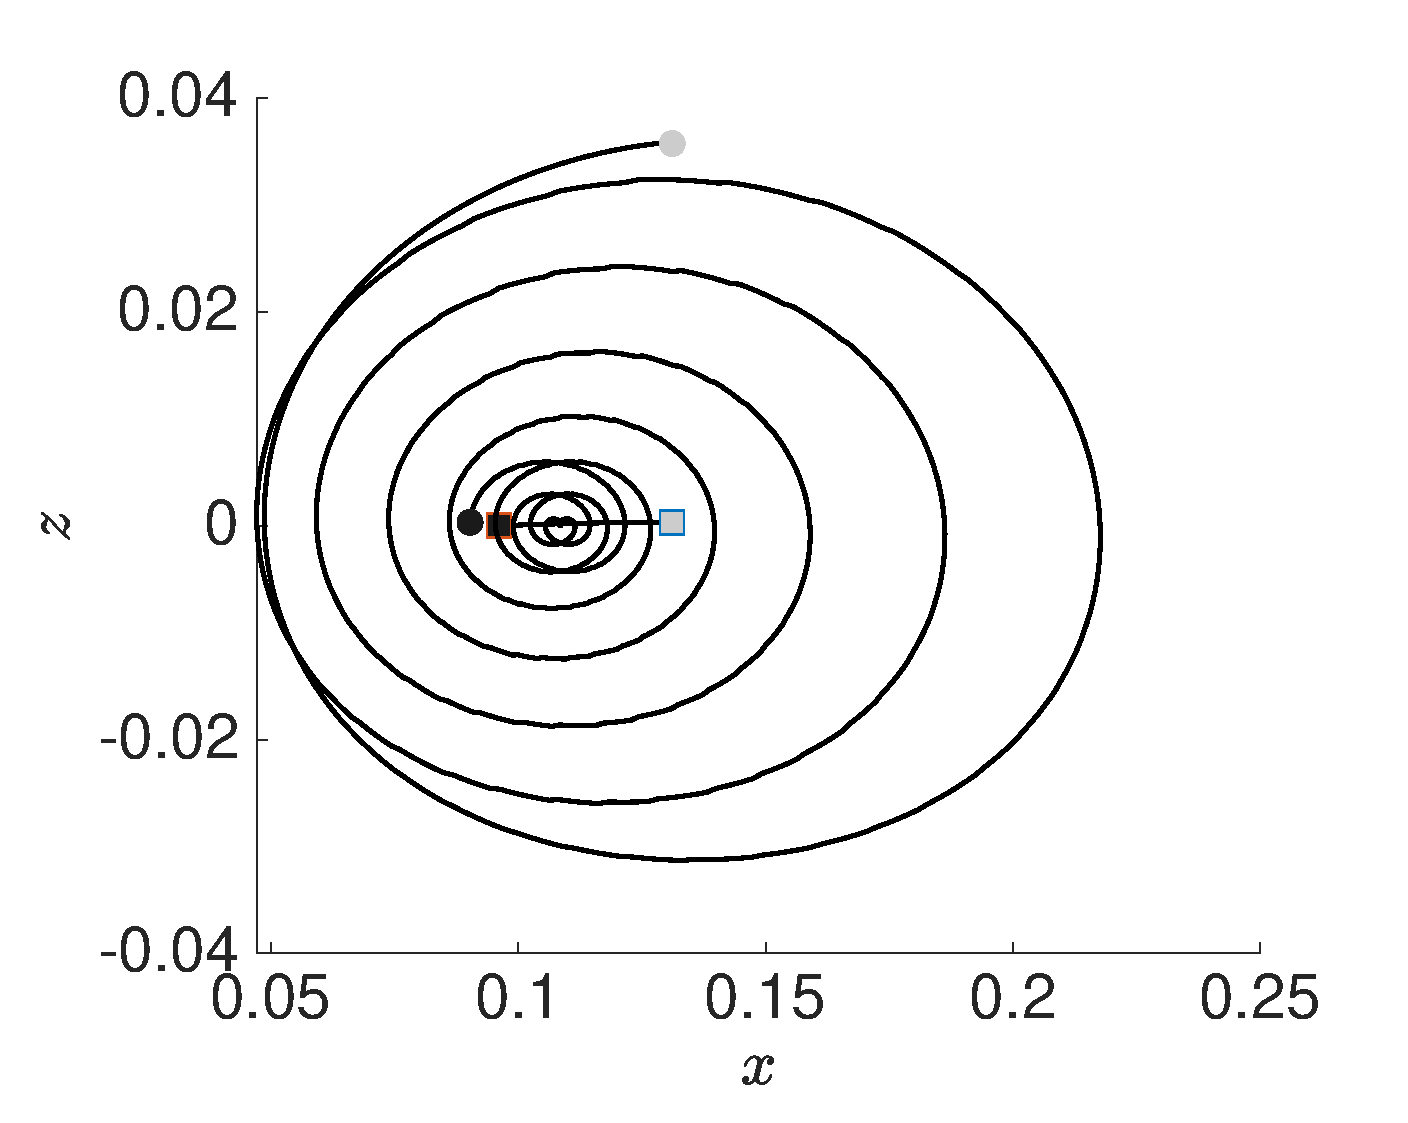
\includegraphics[width=.48\textwidth]{track_ep_pt1_tf_1_w_n1_kap_pt99_foc} & 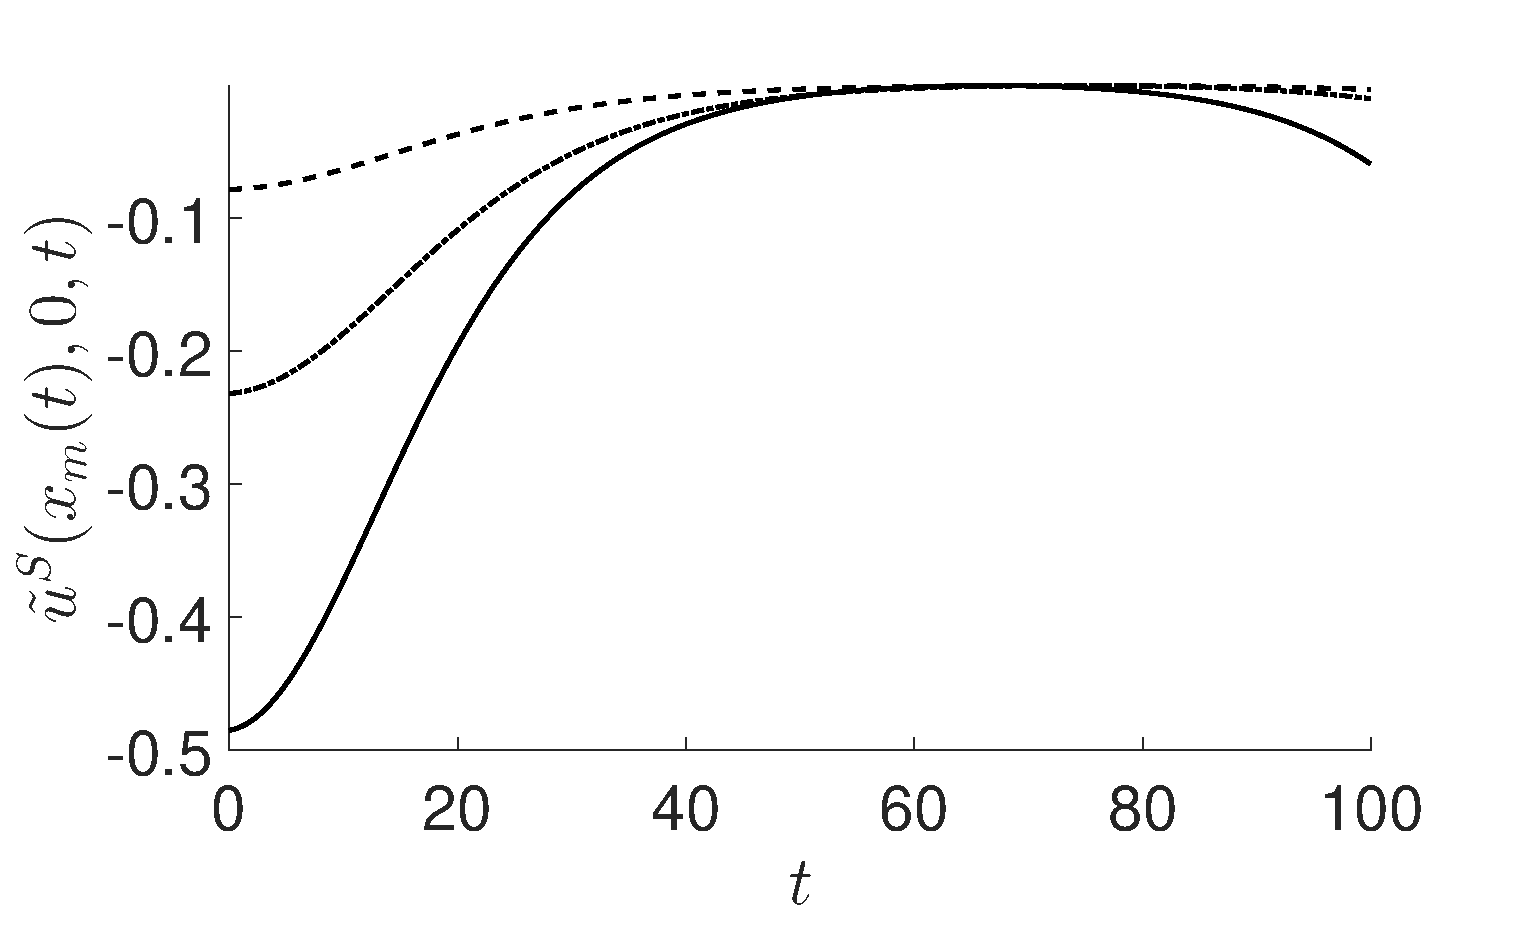
\includegraphics[width=.48\textwidth]{sdrift_comp_ep_pt1_tf_1_kap_pt99_foc}\\
(c) $\omega=-1$ & (d) Stokes Velocity\\
\end{tabular}
\caption{{\bf Focusing} - $k_{0}=1$, $\kappa=.99$, $\omega=0$ (a), $\omega=1$ (b), and $\omega=-1$ (c), Stokes velocity $\tilde{u}^{S}$ (d), where $\omega=0$ (--), $\omega=1$ (-.), and $\omega=-1$ (- -). The grey dot indicates the starting position of the tracer while the black dot indicates the final position.}
\label{fig:foc_kap_pt99}
\end{figure}

Going towards the case of a solitary surface wave, similar results hold for $\kappa=.99$, though we note that the magnitude of particle path oscillations and the Stokes velocity are markedly larger for the larger choice of elliptic modulus; see Figures \ref{fig:foc_kap_pt99} (a)-(d).  What is particularly striking though, as seen in Figure \ref{fig:foc_kap_pt99} (b), is that the counter-propagating shear current is strong enough to create a net rightward drift of the surface particle as well as a strong deformation of the particle path as compared to the $\omega=0$ case seen in Figure \ref{fig:foc_kap_pt99}.  However, the Stokes velocity is still non-positive, see Figure \ref{fig:foc_kap_pt99} (d).  This reflects that the tendency of the particle is still to drift left, but the counter-propagating shear current is able to move the particle strongly to the right when the amplitude of the wave is small.  While counter-intuitive, we note that the leading order shear current is not accounted for in the computation of the Stokes velocity, again due to it being a common term in both the Lagrangian and Eularian mean velocities.  

%%%%%%%%%%%%%%%%%%%%%%%%%%%%%%%%%%%%%%%%%%%%%%%%%%%%%%%%%%%%%%%%%%%%%%%%%%%%%%%%%%%
\subsection{Defocusing Case}
We first study the case of plain waves in the absence of MIs.  To do so, we choose $k_{0}=1$ and $\omega=20$.  As noted previously, only with strong sheer currents can MIs be suppressed at relatively low carrier wave numbers.  For $k_{0}=1$, we can characterize the impact of the shear by noting that $\alpha_{nl}(1,20)\approx40.025$.  Thus, we anticipate a highly oscillatory plane wave pattern, thereby inducing more complicated particle motions and Stokes drift profiles.  Choosing $A=1$ and $\epsilon=.1$, these predictions are borne out by observing the result in Figure \ref{fig:defoc_pwave}.  Here, the simulations are run up to time $t=1/\epsilon = 10$.  Longer simulations make for difficult to interpret graphs which do not fundamentally alter the result.  
\begin{figure}
\centering
\begin{tabular}{c}
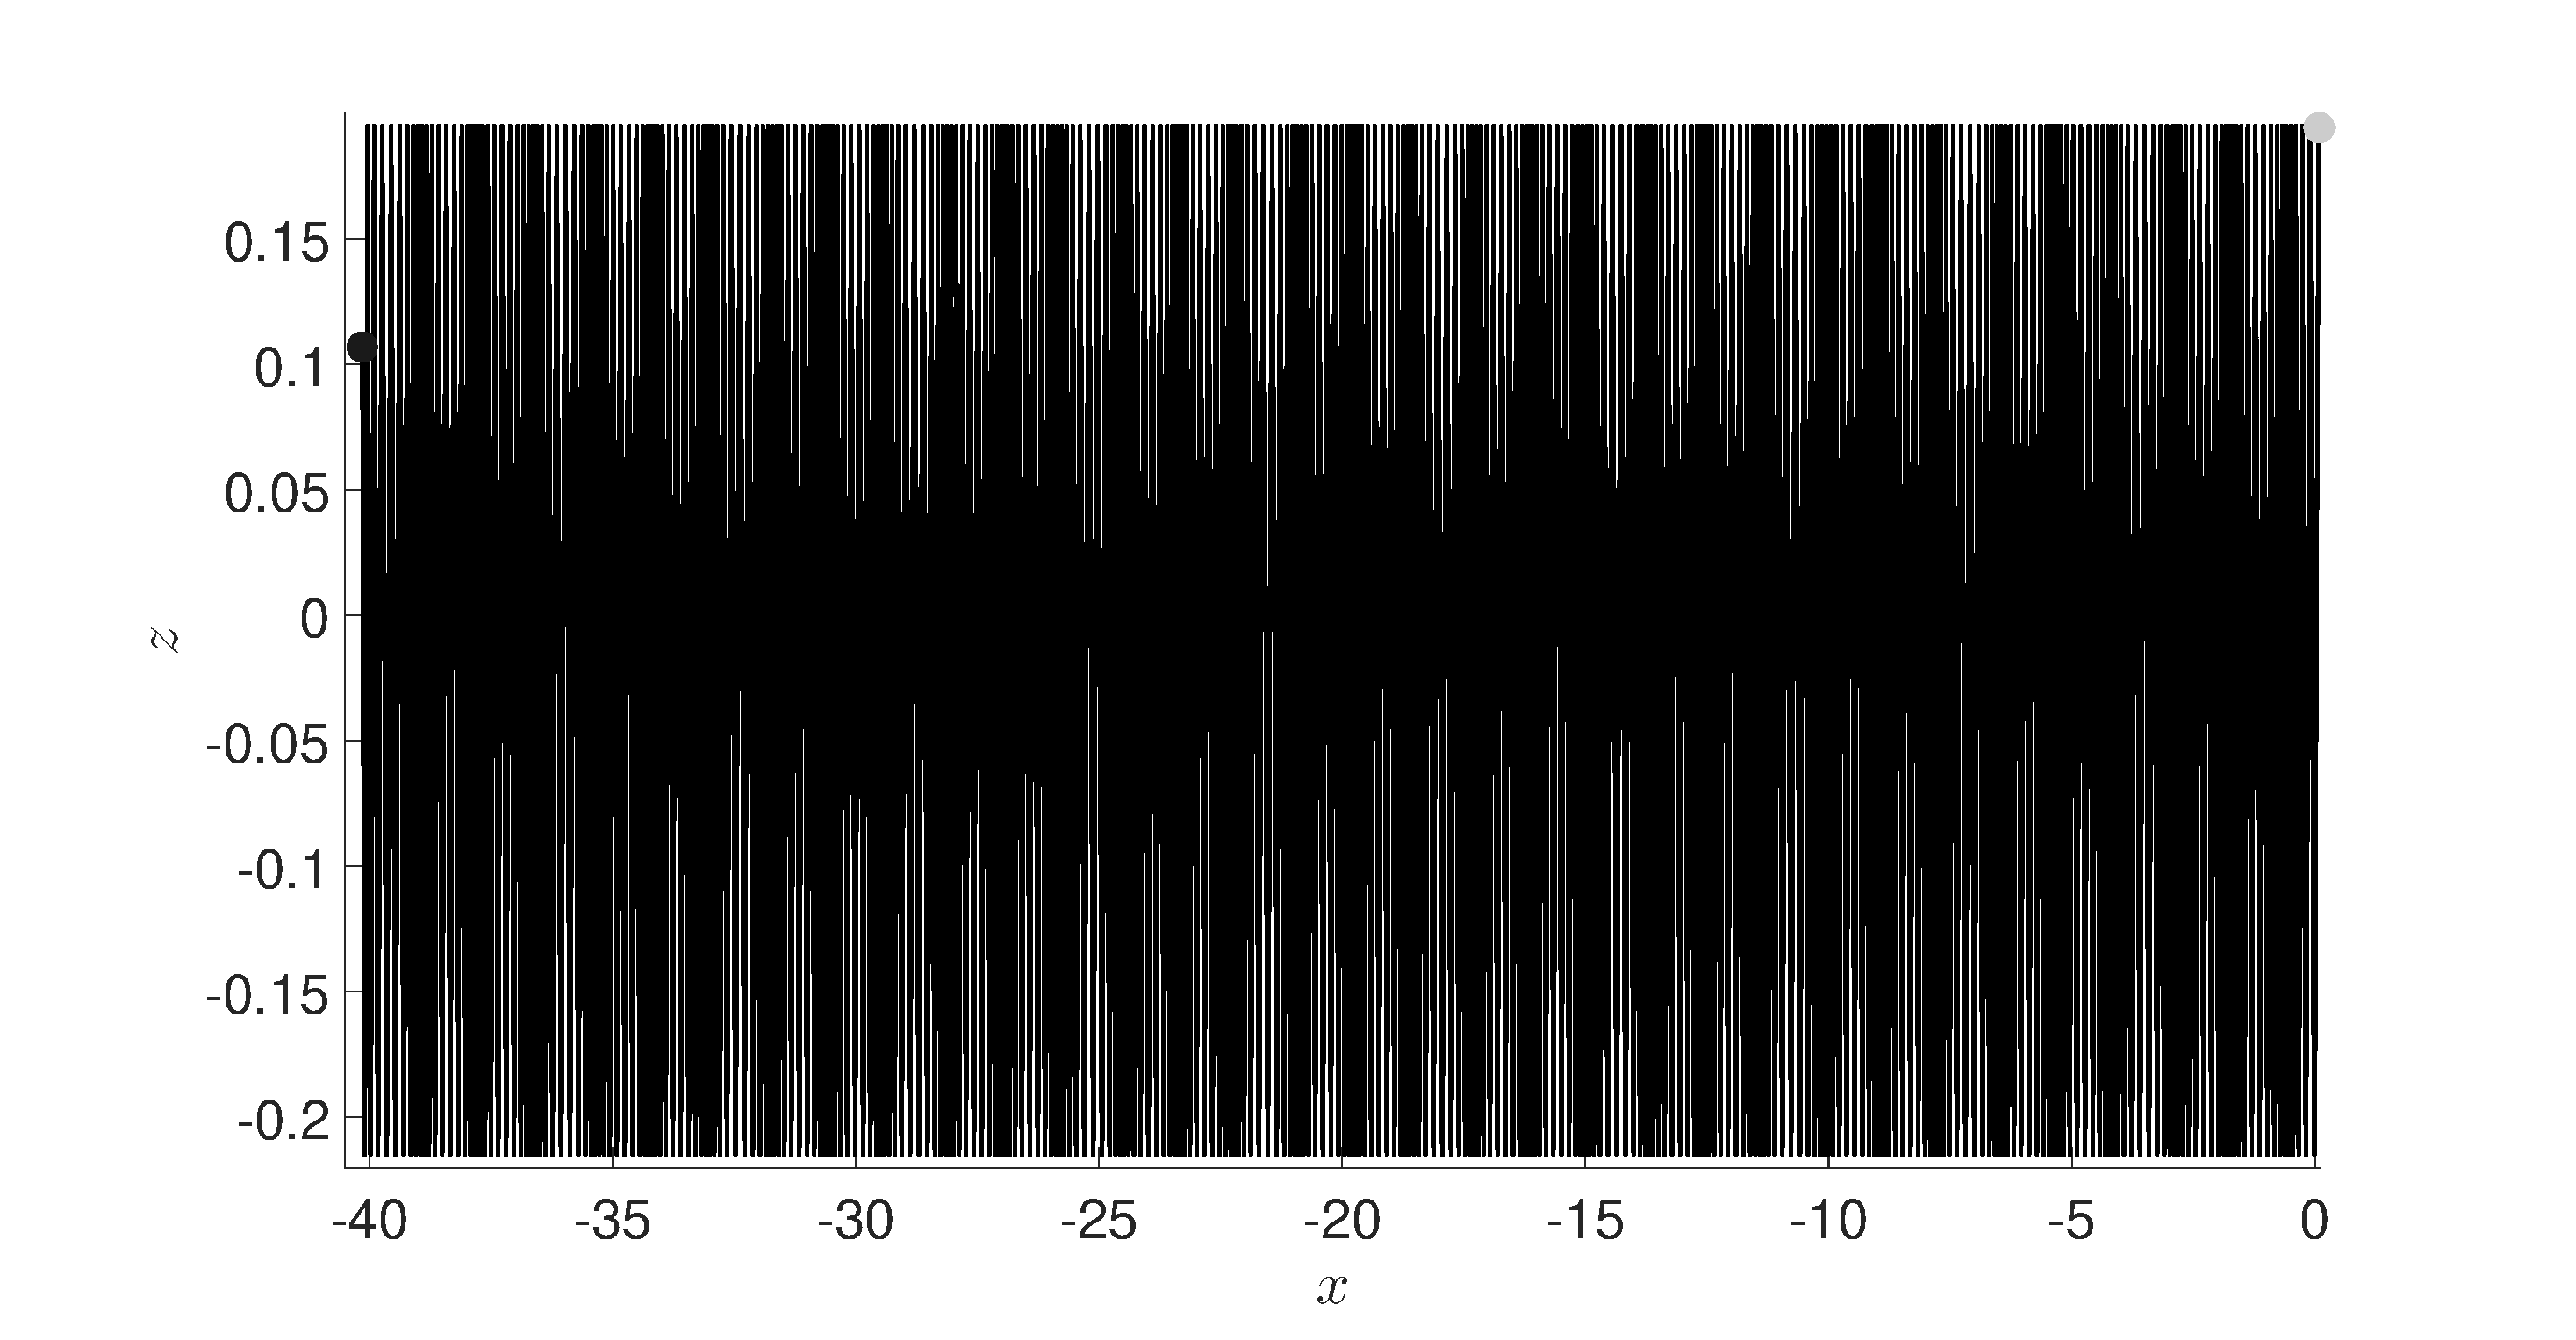
\includegraphics[width=.48\textwidth]{om_val_20_k0_1_ep_pt1_defoc_ztrack_pwave} 
\end{tabular}
\caption{{\bf Defocusing} - Plane wave solution for $k_{0}=1$, $\omega=20$, $A=1$.  The grey dot indicates the starting position of the tracer while the black dot indicates the final position.}
\label{fig:defoc_pwave}
\end{figure}
As seen, the highly oscillatory plane wave profile induces a complicated particle path; see Figure \ref{fig:defoc_pwave}.  Likewise, using Equation \eqref{pwavesdrift}, we can show that the associated Stokes drift velocity at the surface for the plane wave with our given parameter choices is given by 
\[
\tilde{u}^{S}(x,0,t) = -.396  + \mathcal{O}(\epsilon),
\]
which explains the net leftward drift of the particle as seen in Figure\ref{fig:defoc_pwave}. Note, to be asymptotically consistent, we evaluate the Stokes drift velocity at $z=0$ instead of $z=\epsilon \eta(x,t)$.

We now study the defocusing Jacobi elliptic NLS solutions in Equation \eqref{snsolns}.  This is however a less interesting case as can be seen by the plot of $\sqrt{2|\alpha_{d}/\alpha_{nl}|}$ in the defocusing regime in Figure \ref{fig:defoc_amp}.  The characteristic amplitude sizes are on the order of $10^{-3}$ or smaller, and thus the defocusing Jacobi elliptic solutions necessarily correspond to relatively small amplitude profiles.  
\begin{figure}
\centering
\begin{tabular}{c}
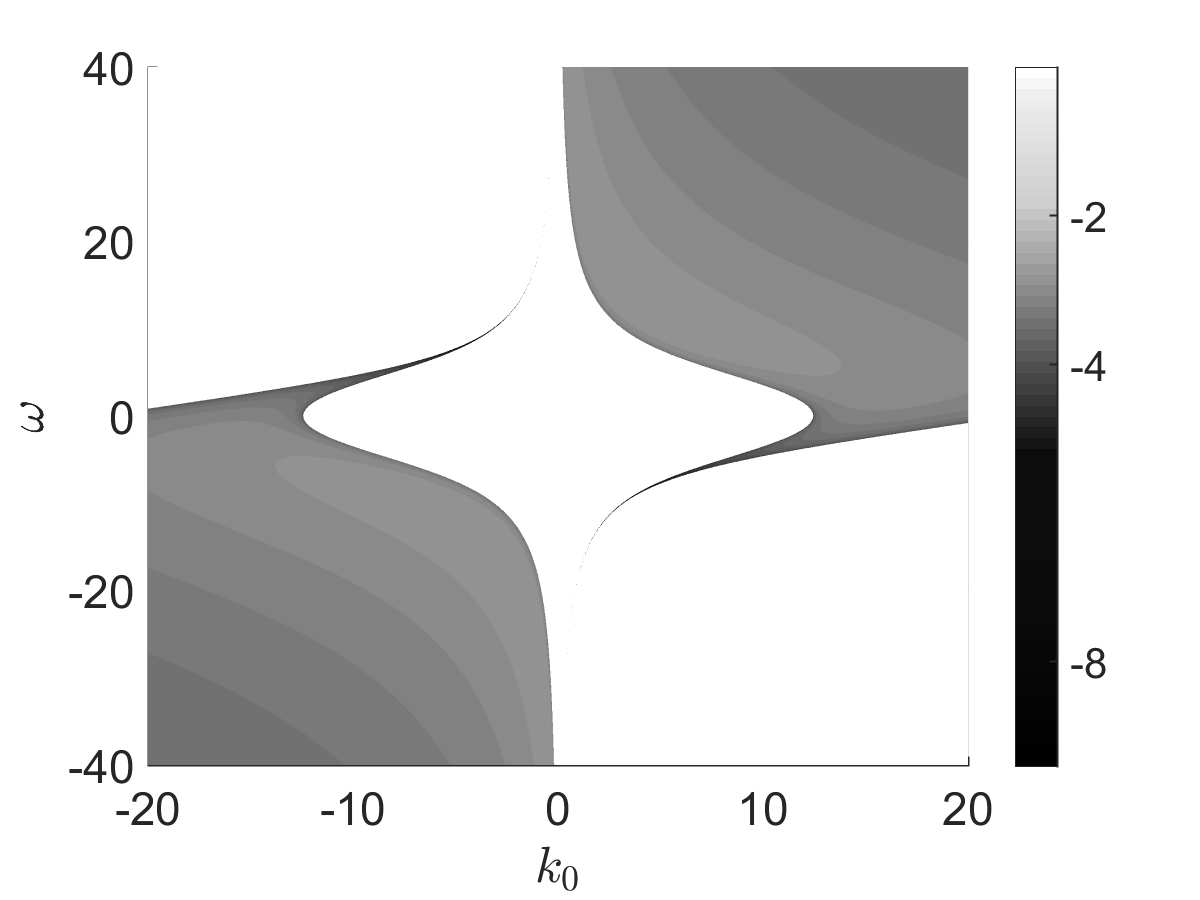
\includegraphics[width=.48\textwidth]{defocusing_ampvals} 
\end{tabular}
\caption{{\bf Defocusing} - Plot of $\sqrt{2|\alpha_{d}/\alpha_{nl}|}$ in the defocusing regime of the NLS equation.}
\label{fig:defoc_amp}
\end{figure}

To illustrate the impact of this weak amplitude via a particular case, we again choose $k_{0}=1$ and $\omega= 20$.  Setting $\epsilon=.1$, and by solving the dynamical system for the particle paths up to time $t=1/\epsilon^{2}$, in the dark-soliton limit with $\kappa=.99$, we generate Figure \ref{fig:defoc_kap_pt99}.  Given that for our particular parameter choices that 
\[
\sqrt{2\left|\frac{\alpha_{d}}{\alpha_{nl}}\right|} \approx 1.13 \times 10^{-3},
\]
we can then readily see why the overall amplitudes of the associated particle path, see Figure \ref{fig:defoc_kap_pt99} (a), and the Stokes drift velocity, see Figure \ref{fig:defoc_kap_pt99} (b), are so small.  Further, while the particle path motion seen in Figure \ref{fig:defoc_kap_pt99} (a) is rapidly oscillating, the net transport is quite weak.  Thus, defocusing Jacobi elliptic solutions would not appear to be as relevant in physical contexts as the defocusing plane wave solutions studied above.   
\begin{figure}
\centering
\begin{tabular}{cc}
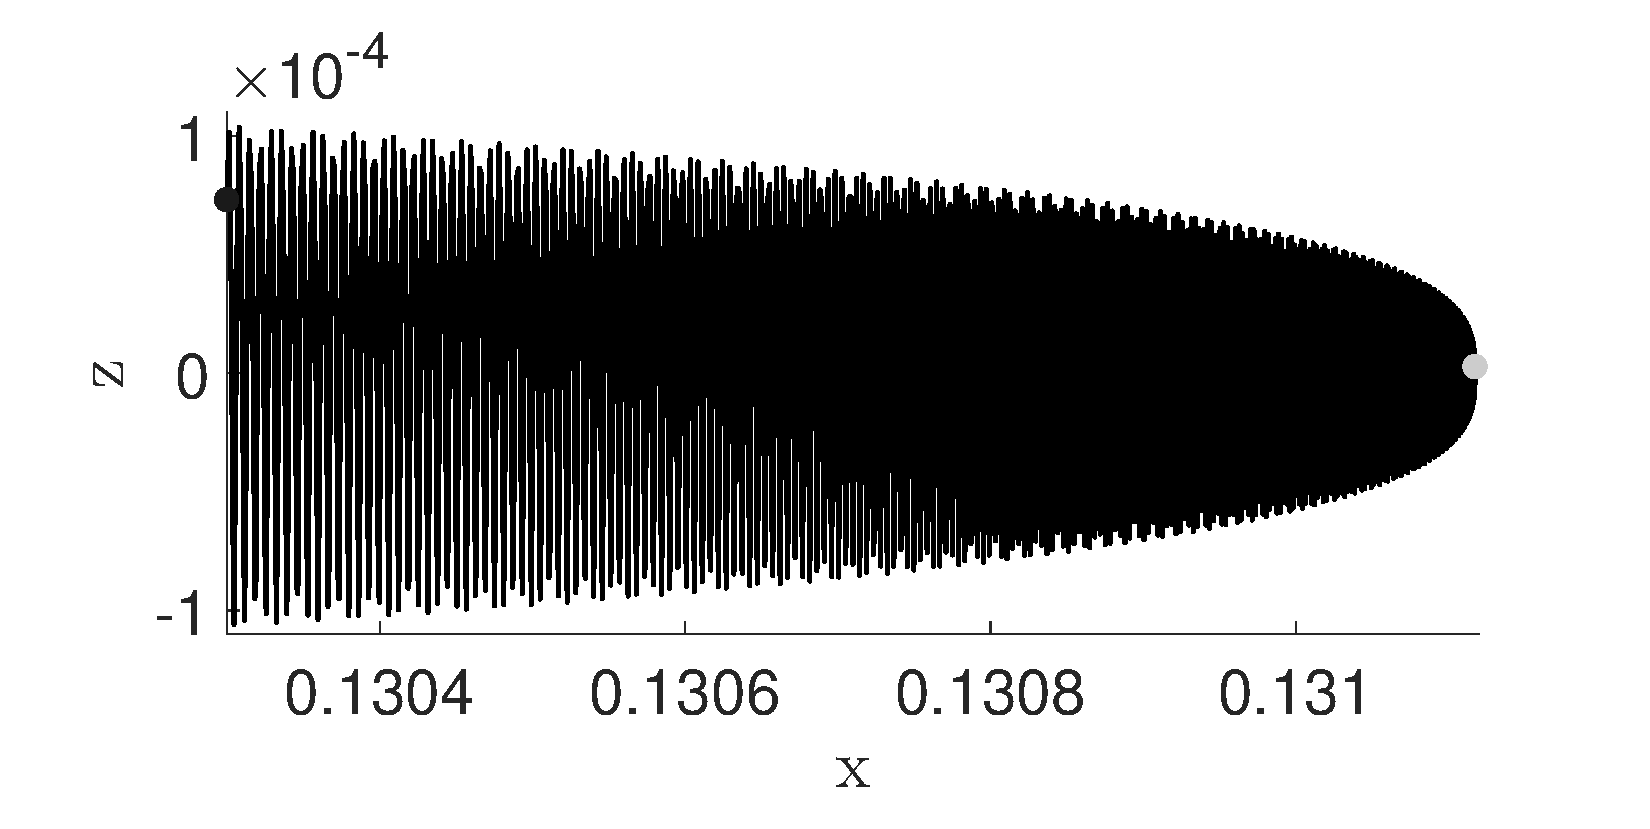
\includegraphics[width=.48\textwidth]{om_val_20_k0_1_ep_pt1_defoc_ztrack} & 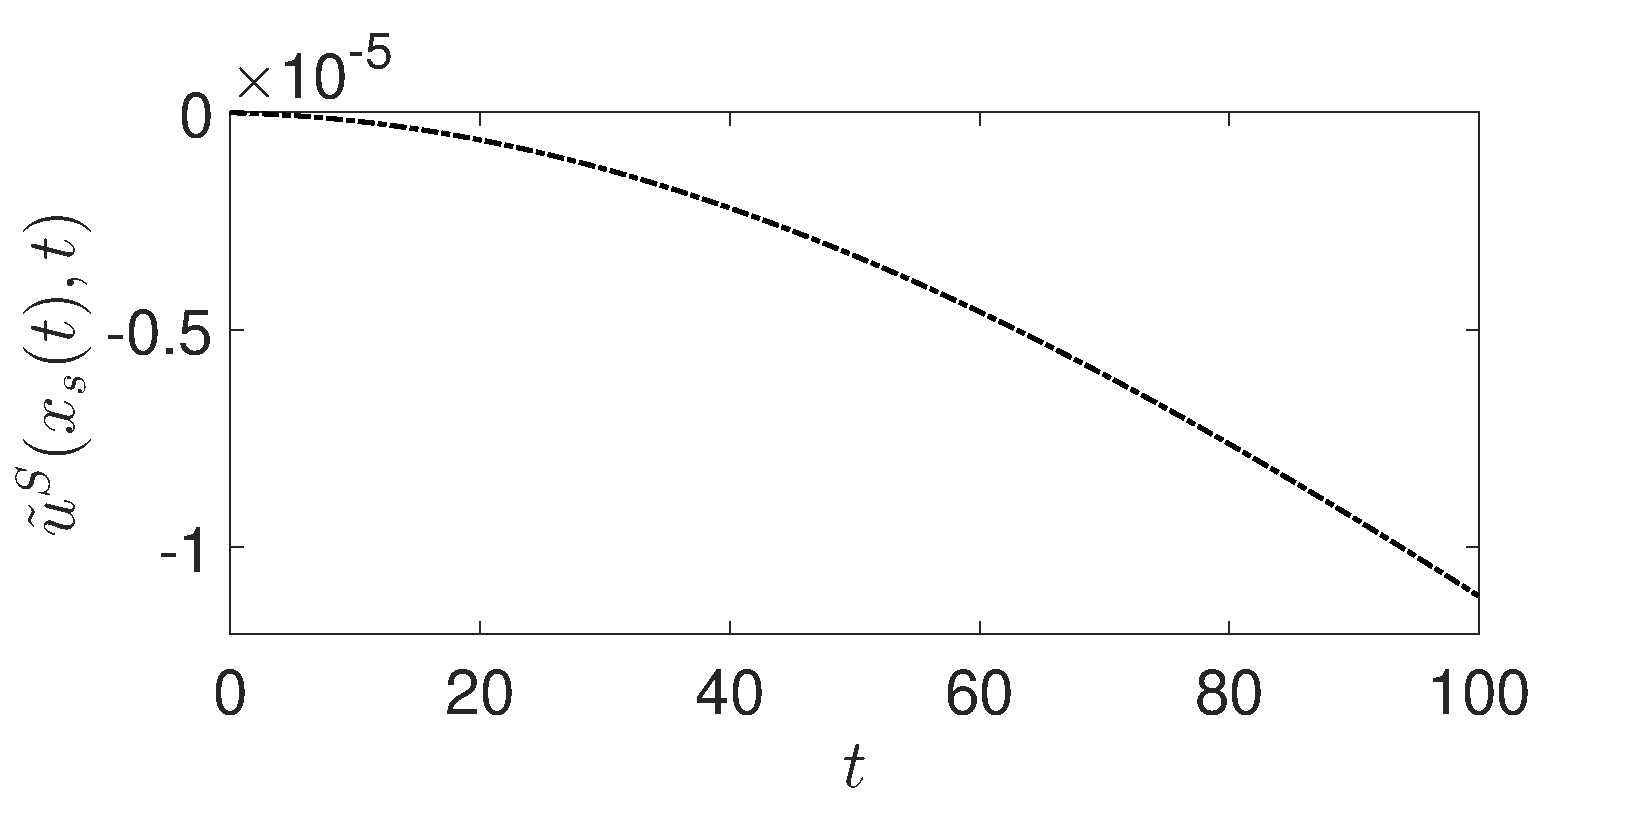
\includegraphics[width=.48\textwidth]{om_val_20_k0_1_ep_pt1_defoc_sdrift} \\
(a) $\omega=20$ & (b) Stokes Velocity\\
\end{tabular}
\caption{{\bf Defocusing} - Near dark soliton solution for $k_{0}=1$, $\omega=20$, $\kappa=.99$ (a), with corresponding Stokes velocity $\tilde{u}^{S}$ (b).  The grey dot indicates the starting position of the tracer while the black dot indicates the final position.}
\label{fig:defoc_kap_pt99}
\end{figure}

%In contrast to this, we look at the case in which $\omega=-20$, which produces the results in Figure \ref{fig:foc_kap_pt99}.  Referring to Figure \ref{fig:miplot} (a), this brings us back to the focusing case, and thus immediately shows the strong modifications that the shear current can have on the surface profile.  Aside from shifting to the focusing case, we see that the strong counter-propagating shear current all but arrests the motion of the surface tracer, and effectively quenches the Stokes drift.  
%\begin{figure}
%\centering
%\begin{tabular}{cc}
%\includegraphics[width=.48\textwidth]{om_val_n20_k0_1_ep_pt1_foc_ztrack} & \includegraphics[width=.48\textwidth]{om_val_n20_k0_1_ep_pt1_foc_sdrift} \\
%(a) $\omega=-20$ & (b) Stokes Velocity\\
%\end{tabular}
%\caption{{\bf Focusing} - $k_{0}=1$, $\omega=-20$, $\kappa=.99$, Stokes velocity $\tilde{u}^{S}$ (b).  The grey dot indicates the starting position of the tracer while the black dot indicates the final position.}
%\label{fig:foc_kap_pt99}
%\end{figure}

%As we would expect, the Stokes velocity, see Figure \ref{fig:defoc_kap_pt5} (d), is positive for all choices of the constant vorticity, reflecting the overall tendency of the waves to travel to the right.  Further, as seen in Figure \ref{fig:defoc_kap_pt5}, the Stokes velocity is significantly reduced in the presence of the counter-propagating shear current.  Again though, the greatest reduction in the Stokes velocity comes from the co-propagating shear current when $\omega=-1$.  This can be explained again by looking at Figure \ref{fig:amfoc}, which plots the term $\sqrt{-2\alpha_{d}/\alpha_{nl}}$ as a function of $\omega$.  As seen, all of the choices of vorticity lessen the amplitude of the function, but the counterpropagating case again causes the greatest loss of amplitude of the NLS solution.  
%\begin{figure}
%\centering
%\includegraphics[width=.48\textwidth]{amp_factor_k0_n1_defoc}
%\caption{The term $\sqrt{2\alpha_{d}/\alpha_{nl}}$ as a function of $\omega$ for $k_{0}=-1$.}
%\label{fig:amdefoc}
%\end{figure}
%Thus, we see that the net rightward drift seen in Figure \ref{fig:defoc_kap_pt5} (c) is due to the shear and the reduction in vertical displacement.  This shear appears then to supresses the rightward drift due to the Stokes velocity when $\omega=0$; see Figure \ref{fig:defoc_kap_pt5} (a) and (d).

%In the limit towards a dark soliton, similar results hold for $\kappa=.99$, though we note that the magnitude of particle path oscillations and the Stokes velocity are markedly larger for the larger choice of elliptic modulus; see Figures \ref{fig:defoc_kap_pt9} (a)-(d).  Again, as seen in Figure \ref{fig:defoc_kap_pt9} (c), we see that the counter-propagating shear current is strong enough to create a significant leftward drift of the surface particle as the amplitude of the carrier wave decreases.  However, the Stokes velocity is still non-positive, see Figure \ref{fig:defoc_kap_pt9} (d).  This reflects the tendency of the particle to drift rightwards, but the counter-propagating shear current is able to move the particle strongly to the left when the amplitude of the wave is small.  

\section{Acknowledgements}
This material is based upon work supported by the National Science
Foundation under Grant No. DMS-1439786 while CC and JC were in
residence at the Institute for Computational and Experimental Research
in Mathematics in Providence, RI, during the Spring 2017 semester.
JC acknowledges and thanks the Norwegian Fulbright Core Scholar
Program for supporting this work.

\bibliography{deep_water_shear}
\bibliographystyle{unsrt}
\end{document}
